%%%%%%%%%%%%%%%%%%%%%%%%%%%%%%%%%%%%%%%%%
% Masters/Doctoral Thesis

% LaTeX Template
% Version 2.5 (27/8/17)
%
% This template was downloaded from:
% http://www.LaTeXTemplates.com
%
% Version 2.x major modifications by:
% Vel (vel@latextemplates.com)
%
% This template is based on a template by:
% Steve Gunn (http://users.ecs.soton.ac.uk/srg/softwaretools/document/templates/)
% Sunil Patel (http://www.sunilpatel.co.uk/thesis-template/)
%
% Template license:
% CC BY-NC-SA 3.0 (http://creativecommons.org/licenses/by-nc-sa/3.0/)
%
%%%%%%%%%%%%%%%%%%%%%%%%%%%%%%%%%%%%%%%%%

%----------------------------------------------------------------------------------------
%	PACKAGES AND OTHER DOCUMENT CONFIGURATIONS
%----------------------------------------------------------------------------------------

\documentclass[
11pt, % The default document font size, options: 10pt, 11pt, 12pt
%oneside, % Two side (alternating margins) for binding by default, uncomment to switch to one side
english, % ngerman for German
doublespacing, % Single line spacing, alternatives: onehalfspacing or doublespacing
%draft, % Uncomment to enable draft mode (no pictures, no links, overfull hboxes indicated)
nolistspacing, % If the document is onehalfspacing or doublespacing, uncomment this to set spacing in lists to single
%liststotoc, % Uncomment to add the list of figures/tables/etc to the table of contents
%toctotoc, % Uncomment to add the main table of contents to the table of contents
parskip, % Uncomment to add space between paragraphs
%nohyperref, % Uncomment to not load the hyperref package
headsepline, % Uncomment to get a line under the header
%chapterinoneline, % Uncomment to place the chapter title next to the number on one line
%consistentlayout, % Uncomment to change the layout of the declaration, abstract and acknowledgements pages to match
the default layout
]{MastersDoctoralThesis} % The class file specifying the document structure

\usepackage[utf8]{inputenc} % Required for inputting international characters
\usepackage[T1]{fontenc} % Output font encoding for international characters
\usepackage{color}
%\definecolor{refC}{rgb}{0.2,0.2,0.6}
\definecolor{refC}{rgb}{0.1,0.1,0.55}
\usepackage[colorlinks,linkcolor=refC]{hyperref}
\usepackage[nomain,acronym,postdot, automake]{glossaries-extra}
\makeglossaries
\setabbreviationstyle[acronym]{long-short}
\loadglsentries{glossy}


%\usepackage{hyperref}
%\hypersetup{colorlinks=true, linkcolor=blue}
%\makeatletter
%\renewcommand\chapter{\addtocontents{toc}{\protect\addvspace{0\p@}}%
%  \if@openright\cleardoublepage\else\clearpage\fi
%  \thispagestyle{plain}%
%  \global\@topnum\z@
%  \@afterindentfalse
%  \secdef\@chapter\@schapter}
%\renewcommand\section{\addtocontents{toc}{\protect\addvspace{0\p@}}%
%  \@startsection {section}{1}{\z@}%
%  {-15ex \@plus -10ex \@minus -10ex}%
%  {13ex \@plus.2ex}%
%  {\normalfont\bfseries}}
%\makeatother

\usepackage{mathpazo} % Use the Palatino font by default

\usepackage[backend=bibtex,style=authoryear,natbib=true]{biblatex} % Use the bibtex backend with the authoryear citation style (which resembles APA)

\addbibresource{example.bib} % The filename of the bibliography

\usepackage[autostyle=true]{csquotes}
\usepackage{graphicx} % Required to generate language-dependent quotes in the bibliography
\usepackage{float}

%----------------------------------------------------------------------------------------
%	MARGIN SETTINGS
%----------------------------------------------------------------------------------------

\geometry{
	paper=a4paper, % Change to letterpaper for US letter
	inner=2.5cm, % Inner margin
	outer=3.8cm, % Outer margin
	bindingoffset=.5cm, % Binding offset
	top=1.5cm, % Top margin
	bottom=1.5cm, % Bottom margin
	%showframe, % Uncomment to show how the type block is set on the page
}

%----------------------------------------------------------------------------------------
%	THESIS INFORMATION
%----------------------------------------------------------------------------------------

\thesistitle{Applied Research of an End-to-End Human Keypoint Detection Network with Figure Ice Skating as Application Scope} % Your thesis title, this is used in the title and abstract, print it elsewhere with \ttitle
\supervisor{Prof. Dr. J. \textsc{Maucher}\\Prof. Dr. S. \textsc{Radicke}} % Your supervisor's name, this is used in the title page, print it elsewhere with \supname

\examiner{} % Your examiner's name, this is not currently used anywhere in the template, print it elsewhere with \examname
\degree{Master of Science} % Your degree name, this is used in the title page and abstract, print it elsewhere with \degreename
\author{Nadin-Katrin \textsc{Apel}} % Your name, this is used in the title page and abstract, print it elsewhere with \authorname
\addresses{} % Your address, this is not currently used anywhere in the template, print it elsewhere with \addressname

\subject{Computer Sciences and Media} % Your subject area, this is not currently used anywhere in the template, print it elsewhere with \subjectname
\keywords{} % Keywords for your thesis, this is not currently used anywhere in the template, print it elsewhere with \keywordnames
\university{\href{http://www.hdm-dtuttgart.de}{Stuttgart Media University}} % Your university's name and URL, this is used in the title page and abstract, print it elsewhere with \univname
\department{\href{https://www.hdm-stuttgart.de/en/prospective_students/academic_programs/all_programs/steckbrief?sgang_ID=550058}{Computer Science and Media}} % Your department's name and URL, this is used in the title page and abstract, print it elsewhere with \deptname
\group{\href{http://researchgroup.university.com}{Research Group Name}} % Your research group's name and URL, this is used in the title page, print it elsewhere with \groupname
\faculty{\href{http://faculty.university.com}{}} % Your faculty's name and URL, this is used in the title page and abstract, print it elsewhere with \facname

\AtBeginDocument{
\hypersetup{pdftitle=\ttitle} % Set the PDF's title to your title
\hypersetup{pdfauthor=\authorname} % Set the PDF's author to your name
\hypersetup{pdfkeywords=\keywordnames} % Set the PDF's keywords to your keywords
}

\begin{document}

\frontmatter % Use roman page numbering style (i, ii, iii, iv...) for the pre-content pages

\pagestyle{plain} % Default to the plain heading style until the thesis style is called for the body content

%----------------------------------------------------------------------------------------
%	TITLE PAGE
%----------------------------------------------------------------------------------------

\begin{titlepage}
\begin{center}

\vspace*{.06\textheight}
{\scshape\LARGE \univname\par}\vspace{1.5cm} % University name
\textsc{\Large Master Thesis}\\[0.5cm] % Thesis type

\HRule \\[0.4cm] % Horizontal line
{\huge \bfseries \ttitle\par}\vspace{0.4cm} % Thesis title
\HRule \\[1.5cm] % Horizontal line

\begin{minipage}[t]{0.4\textwidth}
\begin{flushleft} \large
\emph{Author:}\\
\href{http://nadin-katrin.de/}{\authorname} % Author name - remove the \href bracket to remove the link
\end{flushleft}
\end{minipage}
\begin{minipage}[t]{0.4\textwidth}
\begin{flushright} \large
\emph{Supervisor:} \\
\href{https://www.hdm-stuttgart.de/csm/studiengang/team/professoren}{\supname} % Supervisor name - remove the \href bracket to remove the link
\end{flushright}
\end{minipage}\\[2.2cm]

\vfill

\large \textit{A thesis submitted in fulfillment of the requirements\\ for the degree }\\[0.2cm] % University requirement text
\huge \degreename\\[0.6cm]
\large \deptname\\[0.2cm]
%\today\\[2cm] % Research group name and department name
%\today
\vfill
\textcolor{black}{\large \today}\\ % Date
%\includegraphics{Logo} % University/department logo - uncomment to place it

\vfill
\end{center}
\end{titlepage}

%----------------------------------------------------------------------------------------
%	DECLARATION PAGE
%----------------------------------------------------------------------------------------
\hypersetup{citecolor=refC}
\hypersetup{linkcolor=refC}
\begin{declaration}
	\addchaptertocentry{\authorshipname} % Add the declaration to the table of contents
	\noindent I, \authorname, declare that this thesis titled, \enquote{\ttitle} and the work presented in it are my
	own. I confirm that:

	\begin{itemize}
		\item This work was done wholly or mainly while in candidature for a research degree at this University.
		\item Where any part of this thesis has previously been submitted for a degree or any other qualification at
		\item this University or any other institution, this has been clearly stated.
		\item Where I have consulted the published work of others, this is always clearly attributed.
		\item Where I have quoted from the work of others, the source is always given. With the exception of such
		\item quotations, this thesis is entirely my own work.
		\item I have acknowledged all main sources of help.
		\item Where the thesis is based on work done by myself jointly with others, I have made clear exactly what was
		\item done by others and what I have contributed myself.\\
	\end{itemize}

	\noindent Signed:\\
	\rule[0.5em]{25em}{0.5pt} % This prints a line for the signature

	\noindent Date:\\
	\rule[0.5em]{25em}{0.5pt} % This prints a line to write the date
\end{declaration}

\cleardoublepage

%----------------------------------------------------------------------------------------
%	QUOTATION PAGE
%----------------------------------------------------------------------------------------

\vspace*{0.2\textheight}

\noindent\enquote{\itshape Data is a precious thing and will last longer than the systems themselves.}\bigbreak

\hfill  Tim Berners-Lee
%----------------------------------------------------------------------------------------
%	ABSTRACT PAGE
%----------------------------------------------------------------------------------------

\begin{abstract}
\addchaptertocentry{\abstractname} % Add the abstract to the table of contents
The Thesis Abstract is written here (and usually kept to just this page). The page is kept centered vertically so can expand into the blank space above the title too\ldots
\end{abstract}

%----------------------------------------------------------------------------------------
%	ACKNOWLEDGEMENTS
%----------------------------------------------------------------------------------------

\begin{acknowledgements}
\addchaptertocentry{\acknowledgementname} % Add the acknowledgements to the table of contents
The acknowledgments and the people to thank go here, don't forget to include your project advisor \gls{laser}\ldots
\gls{laser}
\end{acknowledgements}

%----------------------------------------------------------------------------------------
%	LIST OF CONTENTS/FIGURES/TABLES PAGES
%----------------------------------------------------------------------------------------

\begingroup
\hypersetup{linkcolor=refC}
\renewcommand{\baselinestretch}{1.1}\normalsize
\tableofcontents % Prints the main table of contents
\renewcommand{\baselinestretch}{1.5}\normalsize

\printglossaries

\listoffigures % Prints the list of figures

\listoftables % Prints the list of tables

%----------------------------------------------------------------------------------------
%	ABBREVIATIONS
%----------------------------------------------------------------------------------------



\begin{abbreviations}{ll} % Include a list of abbreviations (a table of two columns)

\textbf{LAH} & \textbf{L}ist \textbf{A}bbreviations \textbf{H}ere\\
\textbf{WSF} & \textbf{W}hat (it) \textbf{S}tands \textbf{F}or\\

\end{abbreviations}

%----------------------------------------------------------------------------------------
%	PHYSICAL CONSTANTS/OTHER DEFINITIONS
%----------------------------------------------------------------------------------------

\begin{constants}{lr@{${}={}$}l} % The list of physical constants is a three column table

% The \SI{}{} command is provided by the siunitx package, see its documentation for instructions on how to use it

Speed of Light & $c_{0}$ & \SI{2.99792458e8}{\meter\per\second} (exact)\\
%Constant Name & $Symbol$ & $Constant Value$ with units\\

\end{constants}

%----------------------------------------------------------------------------------------
%	SYMBOLS
%----------------------------------------------------------------------------------------

\begin{symbols}{lll} % Include a list of Symbols (a three column table)

$a$ & distance & \si{\meter} \\
$P$ & power & \si{\watt} (\si{\joule\per\second}) \\
%Symbol & Name & Unit \\

\addlinespace % Gap to separate the Roman symbols from the Greek

$\omega$ & angular frequency & \si{\radian} \\

\end{symbols}

%----------------------------------------------------------------------------------------
%	DEDICATION
%----------------------------------------------------------------------------------------

\dedicatory{For/Dedicated to/To my\ldots}

%----------------------------------------------------------------------------------------
%	THESIS CONTENT - CHAPTERS
%----------------------------------------------------------------------------------------

\mainmatter % Begin numeric (1,2,3...) page numbering

\pagestyle{thesis} % Return the page headers back to the "thesis" style

% Include the chapters of the thesis as separate files from the Chapters folder
% Uncomment the lines as you write the chapters

% Chapter Template


\chapter{Introduction} % Main chapter title

\label{introduction} % Change X to a consecutive number; for referencing this chapter elsewhere, use \ref{ChapterX}
\begin{flushleft}
Human 2D pose estimation has gained more and more attraction in recent years.
For example Facebook, one of the BigFive technology companies, has published 73 research paper targeting the problem of pose estimation in the last three years.
The most popular ones are DensePose and VideoPose3d~\cite{fbPub, DensePose, videopose3d}.
Furthermore, many enterprises are becoming more and more interested in Sport Content Analysis (SPA)
e.g. Bloomberg, SAP and Panasonic, just naming a few~\cite{sappanasonic, spaBloomberg}.
\end{flushleft}
\begin{flushleft}
But how got this topic into such a demanded focal point?
Probably this is due to the various application areas in which Pose estimation can be encountered.
Main fields are sports, visual surveillance, autonomous driving, entertainment, health care and robotics \cite{olympicsport, surveillance, kinectWalkDepression}.
For example Vaak, a japanese startup, developed a software, which would detect shoplifters,
even before they were able to remove items from a store.
This yielded in a drastic reduction of stealing crimes in stores.
\end{flushleft}
\begin{flushleft}
The exercise of Sport not via visiting a sports course, gym or club became of fundamental severance in 2020,
when the Coronavirus SARS-CoV-2 spread the entire world~\cite{coronarki}.
Many courses such as Yoga, Pilates or general fitness routines went online
and were often conducted via Zoom, Instagram live or other video streaming technologies~\cite{coronalife}.
However, what participants were often missing, was the feedback of the coach on how the exercise was going, and whether it was done right or wrong.
So in 2020 more than ever was missed a technology which is good at pose estimation, or even further, action recognition, in sports.
\end{flushleft}
\begin{flushleft}
2D Pose estimation sets the baseline for machines to understand actions.
It is the problem of localizing human joints or keypoints in images and videos.
Many research studies explored and researched this topic already with the most popular ones being OpenPose and VideoPose3d~\cite{openpose, videopose3d}.
A popular company in Canada \textit{wrnch.ai} even specialized on keypoint recognition from image and video data with a lot of product options~\cite{wrnch}.
\end{flushleft}
\begin{flushleft}
For 2D pose recognition there are mainly two general procedures: either top-down or bottom-up.
Top-down first detects a person and then finds their keypoints.
Whereas bottom-up first detects all keypoints in the image and then refers the corresponding people.
For top-down it is argued, that if a person is not detected via a bounding box or alike, no keypoints can be found.
This would lead to more unlabeled frames in a video.
When there are many people in the image with many occlusions the people often can not be detected.
However, when a person is correctly detected, it is said that accuracy would be higher~\cite{synergetic}.
OpenPose, as the famous bottom-up approach, shows results where they were able to detect multiple people with their poses in videos.
With the according hardware this would even show decent results in realtime~\cite{openpose}.
\end{flushleft}
\begin{flushleft}
Most investigations in this field target usual activities not including complex poses which can be encountered in professional sport.
This is why these architectures often fail when applied to more complex movements.
For competitive sports there are various metrics of high interest depending on the environment.
Competition and training can be differentiated as can be sports executed by multiple athletes versus single combats.
Basketball or soccer as team sports for example are interested on predictions about
how the other team behaves during the game and which would be the best reaction to their behaviour for winning the game.
During practice 2d pose recognition can help to optimize the sports-person movements by taking the role of a coach.
This could provide an answer to the question on how certain activities might be optimized? \
Single competitive sports with very complex movement routines are for example gymnastics and figure ice skating.
Both sports include various artistic body movements, which are not part of daily activities.
Even famous and well rated 2d pose recognition networks such as OpenPose or VideoPose3d fail to recognize these poses.
\end{flushleft}
\begin{flushleft}
If this problem was solved it could help with action recognition and support during practice or relieve the jury on competitions.
A predictor could for example suggest, what an athlete should do to land a certain jump.
On the other hand jury is rare and the job sitting all day in the ice-rink on weekends with only a very small salary is not very attractive.
Furthermore, people often complain scoring is not executed fairly.
\end{flushleft}
\begin{flushleft}
Especially in figure ice skating an accurate 2d pose recognition could make a huge contribution.
This is why this paper investigates 2d pose recognition with special focus on figure ice skating.



%----------------------------------------------------------------------------------------
%	SECTION 1
%----------------------------------------------------------------------------------------


%More and more online trainings - corona virus: often via Instagram life or Zoom.
%We as humans can tell whether the person does the movement right or not, so it should be possible for neural networks as well to recognize.
%Everyone has a mobile phone with a camera. No difficult setup needed and no additional hardware.
%
%In some real-world scenarios (e.g. vehicle accidents and criminal activi-
%ties), intelligent machines do not have the luxury of waiting for
%the entire action execution before having to react to the action
%contained in it. For example, being able to predict a dangerous
%driving situation before it occurs; opposed to recognizing it
%thereafte
%
%- profi knowns what action is performed
%    - slow motion: can detect possible errors
%    - put videos next to each other: who jumps higher, turns faster - how fast is difficult
%    - errors difficult to spot -> many ways to land a jump
%- general tasks
%- application areas:
%    - police, games, sports, health
%- in sports
%- figure skating as speciality


%----------------------------------------------------------------------------------------
%	SECTION 1
%----------------------------------------------------------------------------------------


\section{Motivation and Goals}

\begin{flushleft}
A working 2d pose estimator could make a huge contribution to figure ice skating. 
Especially when building an action recognizer on top of it. 
However, as of today, this was not possible yet due to the complex poses and the different gliding movements on the ice.
Especially spins with their fast rotation and stretching poses are of high complexity to these estimators.
Such an estimator could support fair scoring during competitions or help to improve motion sequences during practice.
\end{flushleft}
\begin{flushleft}
With the downward trend of jury staff and the increasing demand for more small competitions, jury is asked more and more in figure ice skating.
Particularly the role of the technical specialist or controller diagnosing the individual elements on the ice is of high demand.
Some competitions were event canceled in recent years, because they were not able to find the according jury.
Furthermore, sitting all day in the cold ice rink for only a very low salary in not attractive at all.
These long demanding days challenge concentration and many competition participants often complain about jury not rating fairly enough,
completely forgetting the demanding work the jury has to do.
Here a 2d pose estimator could contribute by recognizing the different elements or even scoring. 
This would not only relieve the jury but also could increase fairness.
\end{flushleft}
\begin{flushleft}
During practice 2d pose estimators could examine the specific motions during elements and give hints how to improve these.
Probably they could even suggest certain exercises to learn an element like a spin, jump or certain step. 
Additionally they could keep track of training and provide analysis metrics to the skaters and coaches.
\end{flushleft}
\begin{flushleft}
All in all 2d pose estimation is very interesting not only because of all the possible different appliance possibilities in this sport,
 but as well because of the
challenging task to build an according estimator, which was not possible until today.
\end{flushleft}
% - einsatzbereiche - trainer-app, preisrichter-knappheit
% - unger memo
% - große komplexität von eiskunstlauf, fachwissen notwendig
% - keine erfolgreichen studies bis jetzt, neulich veröffentlichtes dataset
% Lorem ipsum dolor sit amet, consectetur adipiscing elit. Aliquam ultricies lacinia euismod. Nam tempus risus in dolor
% rhoncus in interdum enim tincidunt. Donec vel nunc neque. In condimentum ullamcorper quam non consequat. Fusce
% sagittis tempor feugiat. Fusce magna erat, molestie eu convallis ut, tempus sed arcu. Quisque molestie, ante a
% tincidunt ullamcorper, sapien enim dignissim lacus, in semper nibh erat lobortis purus. Integer dapibus ligula ac
% risus convallis pellentesque.


\section{Related Work}

Lorem ipsum dolor sit amet, consectetur adipiscing elit. Aliquam ultricies lacinia euismod. Nam tempus risus in dolor
rhoncus in interdum enim tincidunt. Donec vel nunc neque. In condimentum ullamcorper quam non consequat. Fusce
sagittis tempor feugiat. Fusce magna erat, molestie eu convallis ut, tempus sed arcu. Quisque molestie, ante a
tincidunt ullamcorper, sapien enim dignissim lacus, in semper nibh erat lobortis purus. Integer dapibus ligula ac
risus convallis pellentesque.

% Chapter Template


\chapter{Figure Skating Pose Detection} % Main chapter title

\label{figureskating} % Change X to a consecutive number; for referencing this chapter elsewhere, use \ref{ChapterX}

%----------------------------------------------------------------------------------------
%	SECTION 1
%----------------------------------------------------------------------------------------


\section{Complexity of Figures}
\begin{flushleft}
    Figure ice skating includes very special movement sequences which stand out from other sports.
    Thanks to the surface of the ice, skaters perform gliding movements.
    Furthermore, their programs include highly artisitic
    movements with explosive take-offs, very high rotation speeds and flexible positions.
    Current pose estimators such as OpenPose, VideoPose3d or wrnch.ai all fail to correctly predict
    spins with their high
    rotation speed and difficult flexible positions.
    In this section we try to explain why especially figure ice skating means a challenge in human pose estimation.
\end{flushleft}
\begin{flushleft}
    In single figure ice skating, there are three main element types in a competitive program, which receive
    technical scores:
    jumps, steps, and spins.
    There are seven different listed jumps, which only differ in their take-off phase.
    Three
    of these
    are jumped just from one edge, the Axel, Loop and Salchow.
    The other ones additionally use the skate toe as a catapult.
    Furthermore, they can be distinguished by the edge that is last skated on the ice before the skater takes off.
    This is one of the reasons, why many skaters have problems with the Lutz and Flip jumps.
    For the jury it is often hard to tell as well, weather the jump should get an edge deduction.
    All the jumps can include a different amount of rotation in the air,
    whereas four rotations was the maximum a skater could perform until today.
    All these jumps can be combined in various manners, include features such as lifted arms or difficult steps
    before or after the element to
    increase the level of difficulty, resulting in higher scores.
\end{flushleft}
\begin{flushleft}
    For spins there are four main positions: upright, sit, camel and layback.
    These positions as well can be combined with various features, as for example jumps or difficult elastic positions
    such as the famous Biellmann spin.
\end{flushleft}
\begin{flushleft}
    There are plenty of different step sequence elements including turns on the ice and steps.
    These as well can be combined with multiple additional features resulting in higher scores.

\end{flushleft}
\begin{flushleft}
    The above named elements only explain the absolute basics in figure ice skating.
    In practice scoring and the
    creation of ice skating
    programs is much more difficult.
    Nevertheless, this illustrates nicely, that however for the not professionalized
    audience many elements
    look the same, there are plenty of different metrics and elements.
    Moreover, each skater has their own style
    and performs these elements
    slightly different.
    This is what makes it so hard in machine-learning to correctly predict the elements.
    Which is
    why it is important that
    the basis, the keypoint recognition module, has to predict the poses correctly.
    Because otherwise the action
    recognition module has no
    chance to make correct estimations.
\end{flushleft}
%- existing KP detectors struggle (OpenPose, VideoPose)
%
%Lorem ipsum dolor sit amet, consectetur adipiscing elit. Aliquam ultricies lacinia euismod. Nam tempus risus in dolor
%rhoncus in interdum enim tincidunt. Donec vel nunc neque. In condimentum ullamcorper quam non consequat. Fusce
%sagittis tempor feugiat. Fusce magna erat, molestie eu convallis ut, tempus sed arcu. Quisque molestie, ante a
%tincidunt ullamcorper, sapien enim dignissim lacus, in semper nibh erat lobortis purus. Integer dapibus ligula ac
%risus convallis pellentesque.

%----------------------------------------------------------------------------------------
%	SECTION 2
%----------------------------------------------------------------------------------------


\section{Distinct Rating System}
- isu scores~\cite{isuscores}
- isu guidelines/ level of execution goe~\cite{isuguideleinesgoe}
- human struggle as well -> rating system with points, many abstractions, still often experienced as not fair

Sed ullamcorper quam eu nisl interdum at interdum enim egestas. Aliquam placerat justo sed lectus lobortis ut porta
nisl porttitor. Vestibulum mi dolor, lacinia molestie gravida at, tempus vitae ligula. Donec eget quam sapien, in
viverra eros. Donec pellentesque justo a massa fringilla non vestibulum metus vestibulum. Vestibulum in orci quis
felis tempor lacinia. Vivamus ornare ultrices facilisis. Ut hendrerit volutpat vulputate. Morbi condimentum venenatis
augue, id porta ipsum vulputate in. Curabitur luctus tempus justo. Vestibulum risus lectus, adipiscing nec
condimentum quis, condimentum nec nisl. Aliquam dictum sagittis velit sed iaculis. Morbi tristique augue sit amet
nulla pulvinar id facilisis ligula mollis. Nam elit libero, tincidunt ut aliquam at, molestie in quam. Aenean rhoncus
vehicula hendrerit.

% Chapter Template


\chapter{Dataset} % Main chapter title

\label{Synthetic Dataset} % Change X to a consecutive number; for referencing this chapter elsewhere, use \ref{ChapterX}

%----------------------------------------------------------------------------------------
%	SECTION 1
%----------------------------------------------------------------------------------------


\section{Figure Skating Dataset}

The correct dataset with the according labels is what decides weather a neural network architecture will be able
to sucessfully learn keypoints from image data or video sequence data.
As of today, there does not exist a publicly available dataset which labels keypoints to ice skating performances or
elements.
Famous existing one such as FIS-V or the MIT datasets only include the total technical and performance scores of the
complete performances, which are not applicable her as explained in \autoref{figureskating}.
\\\mbox{}\\
To create a reasonable dataset for figure ice skating there are various possibilities.
Most straightforward would be to make use of the huge amout of vidos published everyday on online platforms such as
YouTube and label the videos by hand. This however would cost a huge amount of time and includes outliers coming from
human errors.
Another possibility would be to work with motion capture.
\\\mbox{}\\
%# Neuron: what is motion capture
%- https://neuronmocap.com/content/mocap-101-what-motion-capture


\subsection{Motion capturing techniques}
There are three main methods for recording motion capturing data.
Markerless capture is a method where videos are recorded via a single or multiple depth cameras.
This comes with the advantage that the athletes are not distracted or feel uncomfortable by any
markers~\cite{mocapopticalradical, mocapopticalcapture, mocapmarkerless3dscans}.
When working with markers there are two sensoring types: optical or inertial.
Optical markers are reflective markers, which are attached to characteristic part of the body.
These reflections are tracked via multiple cameras to make sure the motion movements are taken especially when a
person is moving, so the markers are not concealed~\cite{mocapoptical}.
Inertial motion capture uses IMU sensors that are attached to body parts~\cite{xsens, mocapinterialneuron}.
3D positions then are calculated via multiple sensor metrics.
XSens system for example includes several trackers which contain Magnetometers, gyroscopes and accelerometers.
Via their MVN Animate and Anlaze systems the tracked data is postprocessed on a biomechanical model
and then can be used in game engines such as Unity or Unreal, or in 3D animation software such as Blender or
3DSMax~\cite{xsensabout}.
% https://www.xsens.com/inertial-sensor-modules
% https://www.xsens.com/inertial-sensors
\\\mbox{}\\
In an environment such as the ice rink motion capture has to deal with several difficulties.
For one, the lighting is often not smooth and there are several different light sources.
Moreover, it is very difficult to get the whole ice rink for a recording, because most of the time the ice rink is fully
booked with figure ice skating, ice-hockey, public skating or short track speed skating.
Further, many ice rinks are governed by the local community~\cite{stuttgarteiswelt}, or are highly expensive to rent.
This makes markerless and optical recordings very challenging.
On the other hand inertial recordings as by the XSens technology seem very promising.
Even when there are multiple skaters on the ice, recordings can be tracked in usual practice time slots.

\subsection{XSens: Inertial motion capturing recordings on the ice rink}
In our research study we tested recordings on the ice rink with the MVN Link product from XSens.
This product includes 17 wired IMU motion trackers which can be either attached into a suit or onto straps.
The sensors are connected via cables to a battery whit a life time of 9.5 h.
These trackers are then connected via a router to their MVN Animate software.
The wireless range of the trackers is 50 to 150 meters, however the trackers are able to buffer the recordings
and transmit these later when there is a connection to the hub.
Their MVN Animate software helps with calibration and shows the recording results as soon as the trackers are close
enough
for transmission.
Furthermore, it processes the data and performs adjustments in a postprocessing step~\cite{xsensmvnanimate}.
\\\mbox{}\\
\textbf{Our experiences with MVN Link from XSens}\mbox{}\\
The overall setup was very time consuming. To correctly attach all the straps and align the cables took us a
minimum of 20 minutes. Here we tried out the suit and the straps with equal preparation times.
Then the calibration on the ice with the MVN Analyze software was very time consuming again and took about 20 minutes.
The callibration process had to be repeated several times, when the calibration failed.
These problems probably came from the different gliding movement on the ice.
So the skaters had to mimic usual floor movements for the calibration to work correctly.
Since the recordings are very time consuming we could not work with young professional competitive skaters, because
the setup was too drawn-out.
We then took recordings from a senior competitive skater. The interial method was very beneficial here, because other
skaters on the ice did not intervene in the recordings. Additionally, however sometimes the connection was lost to
the hub, when the skater came back the recordings where transmitted correctly.
The posprocessing from their software did work really good as well.
What was disruptive however, where the sensors and battery, which the skater had to carry.
This made the movements feel constrained. Further, in figure ice skating falls are common.
A fall on the battery or one of the sensors would have been harmful, which again influenced the movement of the
skaters.
In comparison there are other products on the market, that promise a faster setup e.g. through a suit in which the
sensors
are integrated without cables~\cite{mocapinterialneuron}. These products would very likely better fit for figure ice
skating
motion captures.
\\\mbox{}\\
\textbf{Create datset with Blender and MakeHuman}\\\mbox{}\\
We processed the recorded data from the XSens trackers in MVN Animate and then exported a short sequence as bvh file
to test possible dataset creation procedures.
Further, we used the open source MakeHuman~\cite{makehuman} to create a figure skating avatar.
Here we used the figure skating dress and ice skates, which are freely available from the MakeHuman
community~\cite{makehumanassets}.
With the help of the MakeHuman plugin in Blender 2.7~\cite{blender} we then imported the created avatar from MakeHuman
and retargetted the bvh motion capture file onto the rig.
We then set up a default scene with lighting and a moving camera.
To obtain the keypoints, we wrote a Python script in Blender to calculate the joint locations in relation to the camera
view and exported the resulting keypoints into numpy files.
\\\mbox{}\\
However, the above described process seemed to be smooth to conduct, we did face a couple of challenges.
For one, artistic elastic movements yielded in errors on the armature, since the joints were restricted to certain
regions of movement, which seemed to work for usual daily activities but not figure ice skating ones.
Another one was that with the moving camera the keypoints were not calculated correctly and drawn with a small offset.
Recent research studies suggest to export the animation as bvh files and later calculate the joint positions with a
program such as Matlab~\cite{synpose300, 3dpeople, gaitblender}. So this could improve the calculationof joint
positions.
\\\mbox{}\\
\textbf{Our conclusions on creating a synthetic dataset in figure ice skating}\\\mbox{}\\
We are convinced that the above described process to create a synthetic dataset for figure ice skating is a
indispensability when it comes to figure ice skating,
because of the following reasons:\
first: with inertial motion tracking is very accurate espeacially in an environment such as an ice rink when recording
can be easily done during practice sessions.\
second: much less recordings are necessary thanks to the large arbitrary degrees of variation which is possible with
an animation software such as blender\
third: the diversity of data is exceptionally vast.
From one small motion capture file multiple different avatars can be retargetted, female and male, age variations,
clothes and race variances.
Further, multiple different light sources and camera views can be applied and the background randomly selected.\
fourth: calculated labels by the according animation software or post-processing program are just more exact then
human labeled data.
\\\mbox{}\\
All these points confirm the legitimacy of synthetic datasets in figure ice skating.
Which is why we researched on already existing synthetic datasets since in the scope of this thesis creating an own
dataset was not possible due to the huge time efforts.
The systhetic datset 3DPeople as described in the next section correspond our expectations of a synthetic dataset.


%----------------------------------------------------------------------------------------
%	SECTION 2
%----------------------------------------------------------------------------------------


\section{Synthetic Dataset: 3DPeople}

\begin{figure}
    \centering
    \includegraphics[width=130mm]{Figures/woman_step_3dpeople2.png}
    \decoRule
    \caption[3DPeople]{Learned labels from a image sequence of the 3DPeople dataset: Woman stiff walk}
    \label{fig:woman_step_3dpeople}
\end{figure}


The dataset 3DPeople was created via created motion capture files.
They took 70 realistic action sequences from Mixamo~\cite{mixamomotionpac}.
The sequences contain on average 110 frames and range from usual activities with little motions such as driving
or drinking until break dance moves or backflips.
These actions they then retarget onto 80 armatures which are created with MakeHuman~\cite{makehuman} or Adobe
Fuse~\cite{adobefuse}.
There are 40 female and 40 male characters with plenty of variation in body shapes, skin tones, outfits and hair.
Furthermore, they record the actions with a projective camera and 800 nm focal length from four different viewpoints
which are orthogonally aligned with the ground.
The distance to the subjects vary arbitrary as do light sources and static background images.
In sum the dataset includes 22,400 clips with the rendered video sequences as 640x480 pixel image frames, the according
depth maps, optical flow and semantic information such as body parts and cloth labels~\cite{3dpeople}.
\\\mbox{}\\
We found this dataset highly sofisticated due to the wide variance and diversity of the data.
Especially in terms of clothes it stands out from other famous datasets such as Human3.6M~\cite{humaneva}.
They use a variety of wide and tight clothes. For example do they include dresses and shorts.
There variance is greater compared to their freely available combats~\cite{human36m, humaneva}.
In \autoref{fig:woman_step_3dpeople} we demonstrate the learned labels of our modules from a random image of the
3DPeople dataset.



%----------------------------------------------------------------------------------------
%	SECTION 3
%----------------------------------------------------------------------------------------


\section{Data Processing}
The 3DPeople dataset can be recrested through their project homepage and is allowed for use in research
enironments.
Each data package consists of five batches for women and men. There are five data packages available for download.
We created a \textit{data\_admin python class}, which takes care of downloading the data, processing and storing the
data
in memory agnostic and efficient access structured compressed numpy files, and delete the initial downloaded data.
We included several processing steps:
In sum we created four compressed numpy archives.
Every archieve file included an array with all frames of one movement sequence to allow faster reading process for
our neuronal network training later.
The four archives consist of the usual RGB sequence frames, one archive without background, one for the body part
labels,
and one for the joint keypoints.
The numpy archive without background only shows the actors in RGB colors.
Therefore, we used the clothes labels, and replaced all colored pixels with black pixels when the pixels where not
inside the mask.
Initially we did this to test, weather our network ideas would converge with easier data.
Later, when we trained our background-extractor module for getting an end-two-end architecture, this data served as
labels.\\
Furthermore, we cleaned up the body masks and mapped the resulting three dimensional pixels to one-dimensional class
values~\autoref{fig:test21}.
The borders of the body-parts often contained a mixture of RGB values, which where of no use to our network.\\
\begin{figure}

    \fontsmall
\begin{minipage}{0.29\linewidth}
    \begin{Verbatim}[frame=topline,label=Mapping to classes,framesep=1mm]
body_part_classes = {
    BodyParts.bg.name: 0,
    BodyParts.Head.name: 1,
    BodyParts.RUpArm.name: 2,
    BodyParts.RForeArm.name: 3,
    BodyParts.RHand.name: 4,
    BodyParts.LUpArm.name: 2,
    BodyParts.LForeArm.name: 3,
    BodyParts.LHand.name: 4,
    BodyParts.torso.name: 5,
    BodyParts.RThigh.name: 6,
    BodyParts.RLowLeg.name: 7,
    BodyParts.RFoot.name: 8,
    BodyParts.LThigh.name: 6,
    BodyParts.LLowLeg.name: 7,
    BodyParts.LFoot.name: 8
}
    \end{Verbatim}
    \label{fig:test1}
\end{minipage}\hfill
\begin{minipage}{0.49\linewidth}
    \begin{Verbatim}[frame=topline,label=Mapping to RGB values, framesep=1mm]
segmentation_class_colors = {
    BodyParts.bg.name: [153, 153, 153],
    BodyParts.Head.name: [128, 64, 0],
    BodyParts.RUpArm.name: [128, 0, 128],
    BodyParts.RForeArm.name: [128, 128, 255],
    BodyParts.RHand.name: [255, 128, 128],
    BodyParts.LUpArm.name: [0, 0, 255],
    BodyParts.LForeArm.name: [128, 128, 0],
    BodyParts.LHand.name: [0, 128, 0],
    BodyParts.torso.name: [128, 0, 0],
    BodyParts.RThigh.name: [128, 255, 128],
    BodyParts.RLowLeg.name: [255, 255, 128],
    BodyParts.RFoot.name: [255, 0, 255],
    BodyParts.LThigh.name: [0, 0, 128],
    BodyParts.LLowLeg.name: [0, 128, 128],
    BodyParts.LFoot.name: [255, 128, 0]
}
    \end{Verbatim}
     \label{fig:test}
\end{minipage}
    \label{fig:test21}
    \end{figure}
%\begin{figure}
%    \begin{minipage}{10cm}
%        \label{fig:test}
%    \end{minipage}
%\end{figure}



% Chapter Template


\chapter{Method} % Main chapter title

\label{method} % Change X to a consecutive number; for referencing this chapter elsewhere, use \ref{ChapterX}

%learning_rate	0.001
%all_params	3,008,562
%trainable_params	3,003,930
%non_trainable_params	4,632
%layers	156
%training_time_1_epoch	85.43s
%description	Test adam optimizer on hrnet v7

\vspace*{\fill}
\begin{figure}[th]
    \centering
    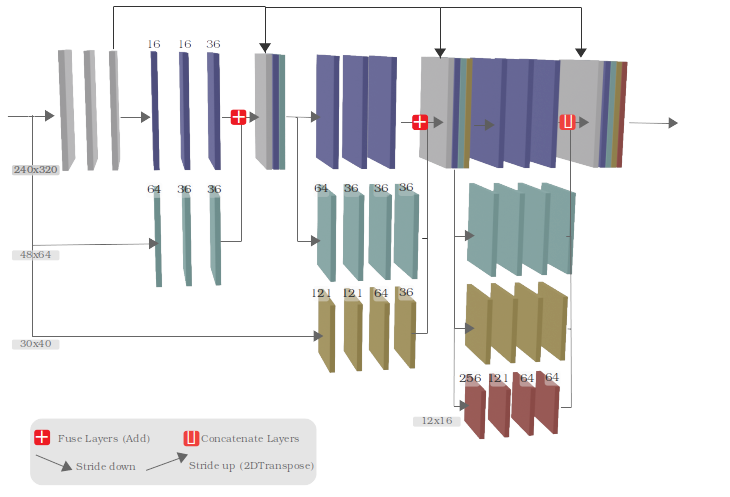
\includegraphics[width=150mm]{Figures/custom_hrnet_lines.png}
    \decoRule
    \caption[HRNetV3: Our HRNet Architecture]{HRNetV3: Our created High-to-low resolution network architecture}
    \label{fig:custom_hrnet}
\end{figure}
For our end-to-end keypoint recognition architecture we have created three modules to extract the background,
find the body parts in the image and detect the human joints or keypoints.
However, to extract the background was not important for other keypoint recognition architectures such as
\textit{OpenPose}~\cite{openpose} or \textit{VideoPose3D}~\cite{videopose3d}, it is important in our architecture, since we wanted
this recognition architecture to be able to be used during practice when there are multiple skaters on the ice,
but only track the focused skater.
With the body part detection module, we altered the well-established approach from \textit{OpenPose} not to recognize vector
fields, which the joints connect, but the visible body parts.
We assume this method to work seamlessly, and estimate that this approach was not chosen before due to the missing
accurate labels for body part detection.
For the keypoint recognition module, we calculate the gaussian with a radius of three pixels and a standard deviation of
three.
In \autoref{fig:alena_step_labeled} we demonstrate an example frame labeled by our three modules
showing Alena Kostornaia, the 2020 European champion during her program.

\begin{figure}
    \centering
    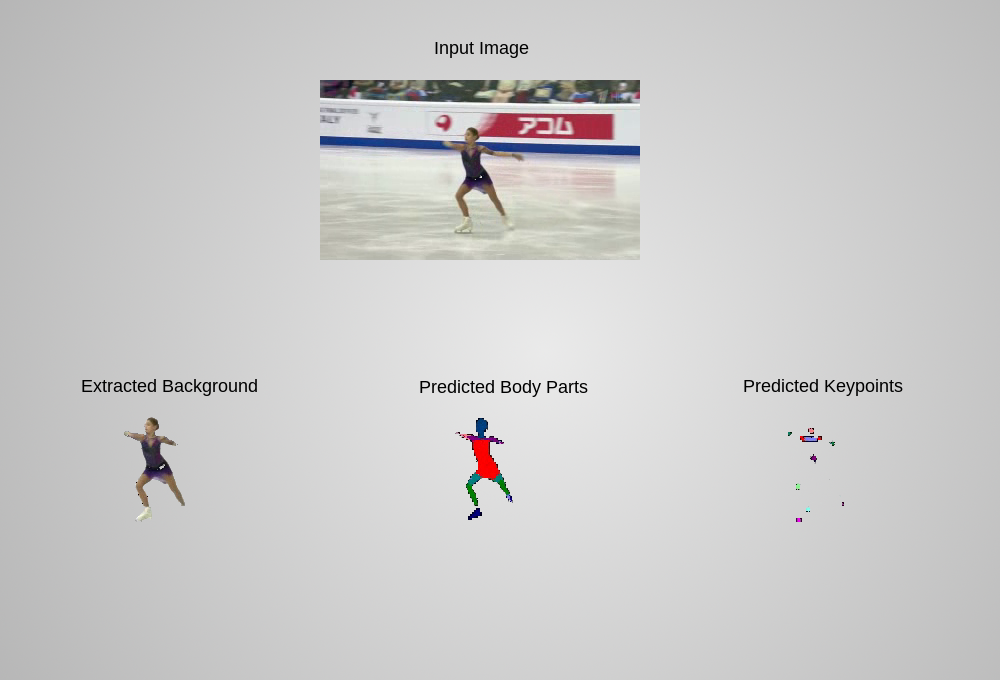
\includegraphics[width=130mm]{Figures/alena_step_labeled2.png}
    \decoRule
    \caption[HRNetV3: Predictions from Alena Kostornaia's Steps]{Learned labels by the three modules: extracted background, human part detection and
    keypoint detection \textit{skater: Alena Kostornaia, 2020 European champion\cite{2020european}}}
    \label{fig:alena_step_labeled}
\end{figure}


All in all, we have built a fully convolutional architecture with three networks, that all are based on high-to-low
representation learning. Our architecture consists of one input block $\mathcal{N}_I$  and three subsequent blocks
$\mathcal{N}_L$, $\mathcal{N}_M$,$\mathcal{N}_S$ and $\mathcal{N}_{XS}$.
These subsequent blocks combine feature maps with lower coarser representations with the original sized input image
feature maps and thus learn the features of the different levels equal to the HRNet strategy~\cite{HRNetv2, HRNetv1}.
\\\mbox{}\\
However, different from the HRNetV1 and HRNetV2 we do not use Pooling to decrease or increase the size of the feature
maps. We decrease the feature maps with usual convolutions and associate strides $\mathtt{s}$ and kernel sizes
$\mathtt{k}$, with $\mathtt{s}=\mathtt{k}$.
To increase the feature maps we use transposed convolutions with again $\mathtt{s}=\mathtt{k}$ according to the
strided down convolutions.
This allows the network to learn additional weights for the upward and downward convolutions and improve these level
exchange processes.
\\\mbox{}\\
Furthermore, we fuse the layer blocks in the first and second stage to combine the mentioned feature levels.
In the third stage, however, we concatenate all feature levels to fully exploit the multi-resolution convolutions
as argued in HRNetV2~\cite{HRNetv2}.
\\\mbox{}\\
As visualized in~\ref{fig:custom_hrnet} we adjusted the number of feature maps for the different blocks.
Moreover, in the first stage, we use only three convolutional layers for one block, in the other stages we use four layers
for the lower levels and only in $\mathcal{N}_L$ we use three convolutional layers for the blocks throughout the network.
\\\mbox{}\\
Another adjustment is, that we use the input image as initial input for all our block levels but the $\mathcal{N}_{XS}$
block, which uses the fused layers of all the other levels as input.
To every stage we add the input block $\mathcal{N}_I$.
\\\mbox{}\\
This network architecture resulted after several experiments and investigations of the estimated feature maps of the
different blocks and stages.
Every block is completed with batch normalization and a \textit{selu} activation function.
The output of the network is predicted by a linear softmax activation function.
For the background-extraction and keypoint detection network we use mean-squared-error as loss function and in the
human part detection network we use a custom loss function~\autoref{Experiments} to optimize the network weights.
In sum, our network comprises 3,008,562 parameters of which 3,003,930 can be learned.
The amount of all layers for one network is 156.\\


% maybe put some images how the different modules did learn

%learning_rate	0.001
%all_params	3,008,562
%trainable_params	3,003,930
%non_trainable_params	4,632
%layers	156
%training_time_1_epoch	85.43s
%description	Test adam optimizer on hrnet v7


%----------------------------------------------------------------------------------------
%	SECTION 2
%----------------------------------------------------------------------------------------


\section{Training Performance (human parts)}
\begin{figure}
    \centering
    \includegraphics[width=130mm]{Figures/hp_accuracy_custom_hrnet_v3.png}
    \decoRule
    \caption[HRNetv3 Training Process: Accuracy]{Improving Accuracy of Training HRNetV3}
    \label{fig:hp_accuracy_hrnet_v3}
\end{figure}
\begin{figure}
    \centering
    \includegraphics[width=130mm]{Figures/hp_loss_custom_hrnet_v3.png}
    \decoRule
    \caption[HRNetv3 Training Process: Loss]{Decreasing Loss  of Training HRNetV3}
    \label{fig:hp_loss_hrnet_v3}
\end{figure}

We trained the human parts module with the Adam optimizer for 5556 episodes, a batch size of 3, and 64 steps per epoch.
One training epoch took on average 85.43 seconds. The whole training lasted about 5.5 days.
For optimization, we have built a custom loss function as explained in
\autoref{Experiments} to better deal with the class invariance of the occurring pixel labels.
The \autoref{fig:hp_accuracy_hrnet_v3} shows, that the accuracy of our network
\autoref{fig:hp_accuracy_hrnet_v3} rises very steep until the 500th episode and then flattens more and more until the last
episode, where the network reaches an excellent accuracy level of 0.99.
In detail, we divided our data into a distinct 90 percent train and 10 percent test dataset.
The figure shows equal trends for both datasets, which means the network did not overfit on the data.\

The loss function in \autoref{fig:hp_loss_hrnet_v3} shows equal opposite trends to the accuracy graph.
It steeply decreases until the 500th episode and then starts to flatten.
Again train and test datasets do not cross each other but show similar courses.

%----------------------------------------------------------------------------------------
%	SECTION 3
%----------------------------------------------------------------------------------------
\section{Inference Runtime Analysis}
The time to predict one frame of size 640x480 pixel takes about 0.3 seconds to run on a Quad-Core Intel i7 CPU with 2.20 GHz,
a simple laptop CPU.
Predictions and training can run on simple hardware as the above mentioned CPU.
The training speed will increase if the minimum version of Cuda
3.5 is supported by the system, since then TensorFlow 2 is able to run on the GPU instead of the CPU.
Due to the age of the named laptop Cuda 3.0 was the highest to be supported.
Since recent developments targeting AI chips in the mobile world by the common companies Apple, Samsung or Huawei,
it is to be expected that the inference of our network does work as well on commonly sold mobile phones today~\cite{mobileAI}.
This sets apart our architecture from \textit{OpenPose}, which we could not use for inference on the mentioned laptop.

%----------------------------------------------------------------------------------------
%	SECTION 4
%----------------------------------------------------------------------------------------
\section{Implementation Details}
We build our Network upon the high-level API TensorFlow 2 which is based on the Keras API~\cite{tensorflow2}.
Our training run on the AI server \textit{J.A.R.V.I.S.} provided by the Stuttgart Media University.
The server contains four Nvidia Titan Xp GPUs with 12 GB RAM and a i7 8-core CPU with 3.2 GHz.
We trained each experiment on a separate GPU. The training was conducted in docker containers using the TensorFlow
\textit{latest-devel-gpu}~\cite{tensorflowdocker} docker build.
The latest TensorFlow docker container did not support Python 3 at the time of this research, but only Python in version
2, which is why we had to use the before mentioned descendant.



% Chapter Template


\chapter{Experiments} % Main chapter title

\label{experiments} % Change X to a consecutive number; for referencing this chapter elsewhere, use \ref{ChapterX}
We conducted several experiments on our human parts and keypoint detection module.
In fact, we applied the resulting network architecture from the human parts module later to the background extraction module.
All in all, we investigated eight network architecture variants differentiating in commonly discussed parameters.
For the keypoint detection module, we conducted tests with and without Dense layers.
On the human parts detection module, we tested the three state-of-the-art optimizers Adam, Nadam, and SGD and experimented with little
modifications to the SGD optimizer.
To overcome class invariance, we tried out three different loss functions under which one we have come up with
ourselves.
In the subsequent sections we will present our experimental setup, results, and constructive thoughts behind the studies.
%----------------------------------------------------------------------------------------
%	SECTION 1
%----------------------------------------------------------------------------------------

% with custom loss function and Adam optimizer_kps


%\section{Different Net Architectures}
\section{Ablation Study}



%-----------------------------------
%	SUBSECTION 1
%-----------------------------------

\begin{table}[]
\begin{footnotesize}
    \caption[Ablation Human Parts Module]{Ablation Human Parts Module: Network Architecture Comparison} \label{table:ablation}
\begin{tabular}{Nlllll}
\hline
\multicolumn{1}{|c}{} &
  \textbf{Name} &
  \textbf{\begin{tabular}[c]{@{}l@{}}Parameter \\ Amount\end{tabular}} &
  \textbf{\begin{tabular}[c]{@{}l@{}}Trainable \\ Parameters\end{tabular}} &
  \textbf{Layers} &
  \textbf{\begin{tabular}[c]{@{}l@{}}Training \\ Time/Epoch\end{tabular}} \\ \hline
\label{HRNet:traditional} & \begin{tabular}[c]{@{}l@{}}HRNet \\ \textit{- traditional}\end{tabular}          & 5,595,221 & 5,589,237 & 171 & 84.76s \\ \hline
\label{HRNet:filter} & \begin{tabular}[c]{@{}l@{}}HRNet \\ \textit{- adjusted filter}\end{tabular}      & 4,936,997 & 4,933,029 & 171 & 66.23s \\ \hline
\label{HRNet:3s} & \begin{tabular}[c]{@{}l@{}}HRNet \\ \textit{- 3 stages}\end{tabular}             & 848,409   & 846,441   & 100 & 82.33s \\ \hline
\label{HRNet:stride} & \begin{tabular}[c]{@{}l@{}}HRNet \\ \textit{- stride-down-up}\end{tabular}       & 4,953,269 & 4,949,157 & 177 & 63.21s \\ \hline
\label{HRNet:stride-i} & \begin{tabular}[c]{@{}l@{}}HRNet \\ \textit{- stride-down-up-input}\end{tabular} & 4,185,605 & 4,181,493 & 177 & 80.57s \\ \hline
\label{HRNet:add-i} & \begin{tabular}[c]{@{}l@{}}HRNet \\ \textit{- add-input}\end{tabular}            & 4,185,605 & 4,181,493 & 177 & 80.57s \\ \hline
\label{HRNet:add-dwconv} & \begin{tabular}[c]{@{}l@{}}HRNet \\ \textit{- add-depthwise-conv}\end{tabular} & 3,182,342 & 3,177,654 & 156 & 83.10s \\ \hline
\label{UNet} & UNet                                                                    & 656,389   & 654,261   & 88  & 85.37s \\ \hline
\label{HRNet:v3} & \begin{tabular}[c]{@{}l@{}}HRNet \\ \textit{- v3}\end{tabular}                   & 3,008,562 & 3,003,930 & 156 & 85.43s \\ \hline
\end{tabular}
    \end{footnotesize}
\end{table}
\setcounter{rowcntr}{0}


\subsection{Body Parts Detection Module }
\label{RBP}

In~\ref{fig:ablation-accuracy} we demonstrate our network architectures, which range from 88 until 177 layers and are
all fully convolutional networks.
For the HRNet \textit{(traditional)}~\ref{HRNet:traditional} we slightly deviate the HRNetV2 presented in~\cite{HRNetv2} by replacing the pooling
layers with strided-down and transposed convolutional layers.
The amount of levels and sizes of the feature maps correspond to~\ref{fig:custom_hrnet}.
As in HRNetV2 we use 4 stages with a filter size of 64 for each stage.
We add one level per stage starting with just the highest level $\mathcal{N}_L$
and concatenate the levels from stage 2 ongoing as demonstrated in HRNetV2.\\
For the HRNet \textit{(filters)}~\ref{HRNet:filter}, we adjust the filters in a way, so that higher levels use fewer filters then lower levels.
Additionally, we decrease the filters from the convolutional layers in the level blocks, starting from the highest filter
amount reducing until 36.
All levels are concatenated with a filter size of 36.\\
Subsequent architectures all make use of the adjusted filter amount.\\
For the HRNet \textit{(3 stages)}~\ref{HRNet:3s}, we only use the three first stages from~\ref{HRNet:filter} and omit
$\mathcal{N}_{XS}$.\
In HRNet \textit{(stide-down-up)}~\ref{HRNet:stride}, we stride down the Input from 240x320x3 to 120x160x36 and use this layer as Input layer
and highest Level $\mathcal{N}_L$. Lower layers scale relatively to $\mathcal{N}_L$.
The HRNet \textit{stride-down-up-input}~\ref{HRNet:stride-i} uses the initially strided down Input layer as input for
every stage instead of the concatenated results for lower levels.\\
As presented in the MobileNet paper~\cite{mobilenet} in~\ref{HRNet:add-dwconv} we experiment with depth-wise convolution
and replace the Concatenation layers after each stage with Add layers.\\
In the UNet~\ref{UNet} we use all levels and combine them via concatenation according to the traditional UNet~\cite{unet}.\\
Finally, we present our resulting high-to-low resolution network HRNet \textit{(v3)}~\ref{HRNet:v3}, where we fuse
the first stages and only concatenate the last stage. Furthermore, we conducted some adjustments to the layer amount
in the levels and stages as presented in~\autoref{method}.
\\\mbox{}\\
The HRNet stride-down-up~\ref{HRNet:stride} seems to train the fastest, when looking at~\ref{fig:ablation-correct-px} the
4.705kth step, it is only at three days and 13h closely followed by the traditional HRNet with the adjusted filters~\ref{HRNet:add-dwconv}
which is at 3 days and 13h. All other trainings took more than four days at that time.
However, one has to keep in mind that both trainings where conducted at the same dates, and the other dates differ.
So the server could have had other workloads, nevertheless, our trainings were the only ones running on the server most
of the time. This occasion as well is reflected in the training time of one epoch.
There as well both the HRNet \textit{stride-down-up} and HRNet \textit{adjusted-filter} only took about ~63, ~66 seconds,
where all the others took more then 80 seconds.
However, we would have expected the U-Net or HRNet \textit{3 stages} to be the fastest since they have the smallest
amount of layers and trainable parameters.
Further, the HRNet \textit{stride-down-up-input} contains less trainable parameters then \textit{stride-down-up}, so
we would have expected a faster training process here.
This verifies that the measurements are dependent from various circumstances.
Indeed, to improve comparability, we measured the third epoch to omit starting warm up phases.
\\\mbox{}\\
\paragraph{Comparison of network architectures}\mbox{}\\
%
The U-Net~\ref{UNet} has the smallest amount of layers with 88 and 654,261 trainable parameters.
The HRNet \textit{stride-down-up}~\ref{HRNet:stride} composes most trainable parameters with 4,949,157 and 177 layers, since the input
layer is first strided down and at the end transposed up again.
On the other hand, due to the reduced feature map sizes, this reduces the computation effort as well.
All comparison figures show very similar curves.
Since we could only run our experiments one complete training each, the results must be viewed circumspectly.
All figures~\ref{fig:ablation-accuracy, fig:ablation-correct-px, fig:correct-pixel-ratio} show very steep curves until
the 500th episode and start to flatten then.\\
When looking at~\ref{fig:train-img-0} and~\ref{fig:train-img-20} this steep initial increase is visually reflected.
When after the first episode the circumferences of the body shapes are predicted vaguely, after the 20th episode the
networks have already learned to predict the locations of body parts relatively close.
Of course, there has to be regarded, that the different predictions were made on different poses, which might differ in
their complexity.
Nevertheless, the UNet~\ref{UNet} and the HRNetV3~\ref{fig:hp_accuracy_hrnet_v3} seem to accomplish superior performance.
After the first episode, the body shape is already estimated precisely close to the input image.
HRNetV3 even shows correct class estimations for different body parts such as the torso, head, arms, and legs already.
In the 20th episode then the labels seem to be estimated very close to the true labels.

\begin{figure}[H]
    \centering
    \includegraphics[width=\textwidth, height=\textheight, keepaspectratio]{Figures/ablation_study_hp_accuracy.png}
    \decoRule
    \caption[Ablation Human Parts Module: Accuracy]{Ablation Human Parts Module: Accuracy Comparison}
    \label{fig:ablation-accuracy}
\end{figure}

The accuracy graph shows that the HRNet \textit{traditional} and HRNetV3 get the best results from epoch 500 onwards.
At step 55.55k they reach 99 percent.
However, the HRNet \textit{stride-down-up} has a lower curve until the 4.3kth epoch, it then makes a jump in Accuracy
and at the end reaches 99 percent as well.
Interestingly the U-Net with the by far fewest parameters and layers does receive very good results as well making almost
99 percent in Accuracy at the end.
The HRNet with only three stages shows the lowest curve and reaches only 98.87 percent points on accuracy at the end.

\begin{figure}[H]
    \centering
    \includegraphics[width=\textwidth, height=\textheight, keepaspectratio]{Figures/ablation_study_hp_correct_pixel.png}
    \decoRule
    \caption[Ablation Human Parts Module: Correct Pixel]{Ablation Human Parts Module: Correct Pixel}
    \label{fig:ablation-correct-px}
\end{figure}

The correct pixel graph~\ref{fig:ablation-correct-px} measures how many pixels of the 240x320 image where labeled correctly
in one batch. The maximum which could be reached here is $240\times320\times3=\numprint{230400}$.
Since the single epochs vary a lot, it makes more sense to look at the smoothed results.
The curves again are very close to each other, with the best results coming from the HRNetV3 with $\numprint{219670}$ and
the HRNet \textit{traditional} with $\numprint{219640}$.
The lowest curve again shows the HRNet \textit{3 stages}.

\begin{figure}[H]
    \centering
    \includegraphics[width=\textwidth, height=\textheight, keepaspectratio]{Figures/ablation_study_hp_bp_pixel_ratio.png}
    \decoRule
    \caption[Ablation Human Parts Module: Correctness Ratio]{Ablation Human Parts Module: Correct Pixel Ratio}
    \label{fig:correct-pixel-ratio}
\end{figure}

For~\ref{fig:correct-pixel-ratio} we summed up the amount of body part pixels and divided by the amount of correctly
predicted pixels for one training batch.
This figure as well displays high variances for the different epochs, which is why it is important to take the smoothed
values into account. We receive similar courses as already inspected in~\ref{fig:ablation-correct-px}.
The HRNet \textit{traditional} and HRNetV3 take the lead wih the \textit{traditional} being slightly above the HRNetV3
with 0.05 percent points. With 31.44 percent the HRNet \textit{traditional} shows the best results, whereas HRNet
\textit{3 blocks} performs worst with 30.38 percent at step 4.93k.

\begin{figure}[H]
    \centering
    \includegraphics[width=\textwidth, height=\textheight, keepaspectratio]{Figures/ablation_study_train_imgs_0.png}
    \decoRule
    \caption[Ablation Human Parts Module: 1st Episode Predictions]{Predicted images of network architectures after first
    episode}
    \label{fig:train-img-0}
\end{figure}
\begin{figure}[H]
    \centering
    \includegraphics[width=\textwidth, height=\textheight, keepaspectratio]{Figures/ablation_study_train_imgs_20.png}
    \decoRule
    \caption[Ablation Human Parts Module: 20th Episode Predictions]{Predicted images of network architectures after 20th
    episode}
    \label{fig:train-img-20}
\end{figure}

\paragraph{Summary}\mbox{}\\
In summary, our experiments show that our constructed HRNetV3 performs best, and the HRNet with only three stages performs
worst.
Interesting here would be different variations in the level of feature map sizes.
For instance what would happen if the level $\mathcal{N}_{XS}$ was maintained as smallest level and the level
$\mathcal{N}_M$ was strided down slightly more?
Insightful as well is the performance of the UNet, which has less than half of trainable parameters and layers compared to
the HRNet \textit{traditional} or HRNetV3, but does not perform much worse.\\
Additionally, further tweaks and studies in these network architectures applied to our different modules would be
greatly enlightening.


%-----------------------------------
%	SUBSECTION 2
%-----------------------------------
\subsection{Joint Detection Module }

\begin{table}[H]

%\begin{footnotesize}
    \caption[Ablation Keypoint Module]{Ablation Keypoint Detection Module: Network Architecture Comparison} \label{table:ablation-kp}
\begin{tabular}{|Nlllll|}
    \hline
\multicolumn{1}{|c}{} &
  \textbf{Name} &
  \textbf{\begin{tabular}[c]{@{}l@{}}Parameter \\ Amount\end{tabular}} &
  \textbf{\begin{tabular}[c]{@{}l@{}}Trainable \\ Parameters\end{tabular}} &
  \textbf{Layers} &
  \textbf{\begin{tabular}[c]{@{}l@{}}Training \\ Time/Epoch\end{tabular}} \\ \hline
\label{kps-dense-blockl} & \begin{tabular}[c]{@{}l@{}}KPS-Dense \\ \textit{- block\_L}\end{tabular}          & 221,748,579 & 218,735,769 & 51 & 68.75s \\ \hline
\label{kps-dense} & \begin{tabular}[c]{@{}l@{}}KPS-Dense\end{tabular}      & 23,097,980 & 20,086,328 & 13 & 67.05s \\ \hline
\label{kps-hrnet} & \begin{tabular}[c]{@{}l@{}}KPS-FCN\end{tabular}             & 4,119,529 & 1,109,991 & 41 & 63.78s \\ \hline
\end{tabular}
    %\end{footnotesize}
\end{table}
\setcounter{rowcntr}{0}

\paragraph{Network Architectures}\mbox{}\\
We created three variations of keypoint detection network architectures of which two\ref{kps-dense, kps-dense-blockl}
utilize Dense layers to estimate the keypoint locations and KPS-FCN~\ref{kps-hrnet} implements the third stage of our
build HRNetV3.\\
KPS-Dense~\ref{kps-dense-blockl}, additionally to the dense stage, utilizes the third stage of the HRNetV3.\\
The dense stage first uses max pooling to reduce the feature map size from 240x230x9 to 120x160x1, 58x78x32, and then 28x38x64.
The resulting pooling layer is flattened and followed by two dense layers, which are combined with AlphaDropout and
batch normalization.
The layers include 1024 and 512 units.
The first Dense layer is connected to a Softmax activation function,
the second to a linear activation function. The model estimates 38 x,y coordinates for the keypoint locations.
The networks loss function calculates the distance from the predicted keypoint locations to the true locations and optimizes
the networks via mean-squared-error.\\
In fact, the KPS-FCN~\ref{kps-hrnet} only uses convolutional layers.
The true labels calculate gaussians with a radius size of three for the locations of the keypoints.
We combined the keypoint classes for equal body locations such has legs and arms, resulting in 11 joint classes.
This network predicts 11 different labels for the classes. The network is optimized as well with mean-squared-error.

All networks are trained with an Adam optimizer and a learning rate of 0.001 and run for 5556 epochs.

\begin{figure}[H]
    \centering
    \includegraphics[width=\textwidth, height=\textheight, keepaspectratio]{Figures/ablation_study_kps_imgs.png}
    \decoRule
    \caption[Ablation Keypoints Detection Module: Predicted Training Images]{Predicted images of keypoint detection networks
    after first, 20th and last episode}
    \label{fig:kps-train-imgs}
\end{figure}

Both figures~\ref{fig:kps-map-loss},~\ref{fig:kps-loss} show similar curves.
Until the 500th episode they decrease steeply and then they start to flatten.
KPS-Dense~\ref{kps-dense} has the fewest layers with 13, however KPS-FCN~\ref{kps-hrnet} contains only 1,109,991
trainable parameters, the dense networks train \~20/ \~218 times more parameters.
The networks only differ slightly in their training epoch time and are all between 63 and 69 seconds.\\
The main difference though is visible in the predicted training images in~\ref{fig:kps-train-imgs}.
The keypoint detection modules seem not to learn the locations of the body parts, but that the probability of the location
of a keypoint being at the center of the image is much more likely than outer locations.
Very interesting about the KPS-FCN is that this network first learns the locations of the feet, and then slowly goes
upward per epoch learning the other keypoint locations in a continuous way.


\begin{figure}[H]
    \centering
    \includegraphics[width=\textwidth, height=\textheight, keepaspectratio]{Figures/ablation_study_kps_map_loss.png}
    \decoRule
    \caption[Ablation Keypoints Detection Module: Loss FCN]{Ablation Keypoints Detection Module: Loss FCN}
    \label{fig:kps-map-loss}
\end{figure}


\begin{figure}[H]
    \centering
    \includegraphics[width=\textwidth, height=\textheight, keepaspectratio]{Figures/ablation_study_kps_loss.png}
    \decoRule
    \caption[Ablation Keypoints Detection Module: Loss Dense Layers]{Ablation Keypoints Detection Module: Loss Dense Layers}
    \label{fig:kps-loss}
\end{figure}

%-----------------------------------
%	SECTION 2
%-----------------------------------
\section{Comparison of Optimizer Algorithms}
\label{optimizers}
\begin{figure}[H]
    \centering
    \includegraphics[width=120mm, height=\textheight, keepaspectratio]{Figures/feature_maps_outpu.png}
    \decoRule
    \caption[HRNetV3: Prediceted Feature Maps]{HRNetV3: Predicted 9 feature map classes of the output layer of the
    human part detection module}
    \label{fig:feature-maps-output}
\end{figure}
Optimizing the weights of a neuronal network is a crucial step in the training life cycle of deep learning.
When our neural network has processed the input image and calculated several feature maps throughout the process,
at the end it predicts 9 feature maps of body parts for example for the head, arms, torso, and legs for the human parts
detection module~\ref{fig:feature-maps-output}.
With the help of a loss function, we then calculate the error for the predicted pixels in comparison to the truly labeled
pixels.
The optimizer updates the network parameters $\theta \in \mathbb{R}^d$, which result in learned filters predicting several feature maps at
the different stages of the network.
The updates are performed accordingly to the calculated error from the loss function $\mathcal{J}(\theta)$ via the
so-called Backpropagation process, since the updates are passed backward through the network.
This backward optimization process is performed by the calculations of the chosen optimizer.
The goal of the optimizer is to minimize the error.
There, it makes use of gradient descent to update the network's weights, biases and activation functions, in opposite direction
of the gradient.\\
Figuratively speaking, a weight could be imagined as a hill.
The updates then will follow the direction of the slope downhill until the valley is reached.
Whereas the valley is equal to a local minimum~\cite{optimizersoverview}.
\\\mbox{}\\
There are three variants for gradient descent:\\
\textbf{Batch Gradient Descent (BGD)}, which calculates the gradients $\theta$ for the entire training dataset.
The problem here is, that most of the time this would not fit into the RAM.
We, for example, had problems with data overflow when we trained with more than 12 images at a time, however, we even reduced
the image size to 320x240.
Another drawback is, that gradients for similar examples must be recalculated before each update, leading in redundant computations.\\
\textbf{Stochastic Gradient Descent (SGD)} confronts this problem by performing updates for each training example input image $x_i$
and mask label $y_i$.
This optimization process is much faster.
Moreover, the updates are of more variance when random training examples are chosen.
A drawback however is, even if jumping around may result in finding another better local minimum, it may also
lead to constantly overshooting the exact minimum.
Against this problem, slowly decreasing the learning rate may help and lead to similar convergence as for BGD.\\
\textbf{Mini-Batch Gradient Descent} is the most common variant for gradient descent since it combines both the aspects of
BGD and SGD.
The updates are conducted for every mini-batch of \textit{n} training samples.
This reduces the variance of parameter updates and leads to less jumping around, which all in all results in more stable
convergence~\cite{optimizersoverview}.
\\\mbox{}\\
In the following section, we will present an overview of optimizers targeting the optimizers we experimented on, which are
SGD, Adam and Nadam.
We conducted our training with Mini-Batch Gradient Descent with a batch size of three.
In addition, we will present some mathematical backgrounds of optimizer algorithms and explain further aspects of
SGD in more detail.

\subsection*{Overview of our used optimizers}
%
\textbf{Stochastic Gradient Descent (SGD)} is one of the first optimizers and still commonly in use.
Already in 1951, it was publicly reported by Robins and Sutton et Al~\cite{sgd}.
Now given the parameters of a neural network $\theta$, such as weights, biases and activation functions, here via an input image
$\mathfrak{x}$ and associate labels $\mathfrak{y}$ the Backpropagation process is defined under the gradient $\nabla$
from the calculated loss function $\mathcal{J}$.
The adaption of the parameters then is performed stepwise by the learning parameter $\eta$.


\begin{equation}
    \theta = \theta - \eta\cdot\Delta_\theta\mathcal{J}(\theta;x;y)
    \label{eqn:sgd}
\end{equation}

The SGD optimizer updates a weight $\mathrm{w}$ in a way to reduce the loss function $\mathcal{J}(\mathrm{w})$ and find
the local minima of the parameters.
As already mentioned, this is one of the problems with pure SGD, since it will very likely become stuck in a local minimum or
saddlepoint, where one slope goes up and the other one down.
Furthermore, it converges slower compared to newer optimizers~\cite{optimizersoverview, optimizersexplained}.
\\\mbox{}\\
\textbf{Momentum}, first proposed in 1999 by Qian et Al.~\cite{momentum}, can help to get faster to the local minimum.
This is accomplished by an additional term that is added to SGD.
A constant fraction $\gamma$ is multiplied with the last parameter update $\mathfrak{v}_t$ to $\theta$.

%\begin{align}
%    \theta_t = \theta_t - \eta * \nabla\mathcal{J}(\theta_{t})+\gamma\mathfrak{v}_{t} \label{eqn:momentum:1}\\
%    \mathfrak{v}_t = \nabla\mathcal{J}(\theta_{t-1})+\mathfrak{v}_{t-1} \label{eqn:momentum:2}\\
%    \theta_t= \theta_t - \eta * \nabla\mathcal{J}(\theta_{t})+\gamma\sum_{\tau=1}^{t}\eta * \nabla\mathcal{J}(\theta_{\tau}) \label{eqn:momentum:3}
%\end{align}
\begin{align}
    \theta = \theta - \mathfrak{v}_t \label{eqn:momentum:1}\\
    \mathfrak{v}_t = \gamma\mathfrak{v}_{t-1} + \eta\cdot\nabla_\theta\mathcal{J}(\theta) \label{eqn:momentum:2}
\end{align}

Since the momentum term includes all previous updates~\ref{eqn:momentum:2}, it allows the optimizer to accelerate in terms of speed towards
the local minimum and thus converge faster.\\
This can be associated with a ball rolling down a hill.
The momentum term increases, as the ball rolls downhill, accelerating in terms of speed for subsequent gradients
which point in the same direction.
When the direction changes, the term decreases, and the ball slows down.
All in all, this results in faster convergence and less oscillation or jumping around the minimum~\cite{optimizersoverview}.
\\\mbox{}\\
\textbf{Adaptive Gradients (AdaGrad)}, a newer algorithm proposed in 2011 by Duchi et Al.~\cite{adagrad},
adapts the size of an update to the importance of the individual parameters.
This is a great benefit for the occurrence of sparse data, which is the case for image data or word embedding tasks.
It adjusts the learning rate term, by dividing the learning rate through the sum
of previous updates w.r.t the network parameter $\theta_i$ at time step t.
An additional smoothing term $\eta$ prevents the division by zero.

\begin{equation}
    \theta_{t+1,i} = \theta_{t,i} - \frac{\eta}{\sqrt{\epsilon+\sum_{t=1}^{t}(\nabla_\theta\mathcal{J}(\nabla_{\theta_{t,i}}))^2}} \cdot \nabla_\theta\mathcal{J}(\theta_{t,i})
    \label{eqn:adagrad}
\end{equation}
This results in the learning rate decreasing when approaching a local minimum, meaning the overshooting problem is eased off.
However, one weakness is the growing dominator, which makes the learning rate shrink to an infinitesimally small number until the step
size almost dissolves to zero.
\\\mbox{}\\
\textbf{Root Mean Squared Propagation (RMSProp)} extends AdaGrad's root squared loss function.
It is an unpublished optimization technique proposed by Hinton et Al.~\cite{rmsprop}.
The dominator takes, additionally to the past squared gradients, the current gradient at the current time step t,
into account, weighting the last update more than the current.
Hinton suggests to weight the last update with 90 and the current with 10 percent.
\begin{align}
    \theta_{t} = \theta_{t-1} - \frac{\eta}{\epsilon+E[g^2]_t} \cdot \nabla_\theta\mathcal{J}(\theta_{t-1})\label{eqn:rmsprop:1}\\
    E[g^2]_t = (1-\gamma)g^2+\gamma E[g^2]_{t-1}\label{eqn:rmsprop:2}\\
    g = \nabla_\theta\mathcal{J}(\theta_{t,i})\label{eqn:rmsprop:3}
\end{align}
Unlike AdaGrad, RMSProp does not decrease monotonously, but can adapt the size of adaption.
Now larger or smaller updates are possible in reference to their impact.
Nevertheless, the issue with diminishing learning rates remains.
\\\mbox{}\\
\textbf{Adaptive Moment Estimation (Adam)}~\cite{adam}, as well as AdaGrad or RMSprop, calculates adaptive learning rates w.r.t. the
the parameters $\theta_i$.
As an extension, it keeps track of an exponentially decaying average of past gradients $m_t$, as was already done in
momentum.\\
Coming back to the visual anecdote, the ball has a lot of weight and is very heavy~\cite{optimizersoverview}.
It prefers flat minima.\\
Past decaying average $m_t$ and past squared errors $v_t$ estimate the first momentum (the mean) and the second momentum
(the uncentered variance).

\begin{align}
    m_t &= \beta_1 m_{t-1} + (1 - \beta_1) g_t \label{eqn:adam:1}\\
    v_t &= \beta_2 v_{t-1} + (1 - \beta_2) g_t^2 \label{eqn:adam:2}
\end{align}

Since these terms are biased with zeroes, the initial updates are very small.
Which is why $\hat{m}_t$ and $\hat{v}_t$ bias these terms:

\begin{align}
\hat{m}_t &= \dfrac{m_t}{1 - \beta^t_1} \label{eqn:adam:3}\\
\hat{v}_t &= \dfrac{v_t}{1 - \beta^t_2} \label{eqn:adam:4}
\end{align}

This results in an update rule which reassembles RMSProp:

\begin{align}
    \theta_{t+1} = \theta_{t} - \dfrac{\eta}{\sqrt{\hat{v}_t} + \epsilon} \hat{m}_t \label{eqn:adam:5}
\end{align}

%However, this term not only takes the gradient into account, but additionally as in RMSProp~\ref{eqn:rmsprop:2} the
%previous updates to the gradient in relation to a constant term $\beta_1$, which again stands in relation to the
%current time step t.
%Equally to the numerator, Adam takes the gradient and previous gradient updates in the dominator into account, which we
%could already observe in~\ref{eqn:rmsprop:1} ff.:
%
%\begin{align}
%    \hat{m}_t = \frac{m_t}{1-\beta_1^t} \label{eqn:adam:2}\\
%    \hat{v}_t = \frac{v_t}{1-\beta_2^t} \label{eqn:adam:3}\\
%    m_t = (1-\beta_1)g_t + \beta_1 m_{t-1} \label{eqn:adam:4} \\
%    v_t = (1-\beta_2)g_t^2 + \beta_2 v_{t-1} \label{eqn:adam:5}
%\end{align}

In particular, Adam makes use of two decay parameters $\beta_1$ and $\beta_2$, referred to as exponential decay rates.
These parameters $\beta_1$ and $\beta_2$ are close to the constant $\gamma$ term used in RMSprop and Momentum.
The great advantage here is, that the learning rate can adapt in both directions solving the issue from AdaGrad or
RMSProp of vanishing learning rates.
\\\mbox{}\\
\textbf{Nesterov-accelerated Adaptive Moment Estimation (Nadam)},
now replaces Momentum with the better performing
Nesterov accelerated gradient (NAG).
It was first presented in 2016 by Dozat et Al~\cite{nadam}.\\
\\\mbox{}\\
\textbf{NAG} allows to approximately calculate the future position of the parameters.
Referring back to Momentum, NAG is like a smarter ball, which knows that it has to slow down and not naively go up an upcoming
slope again just to roll back down.
NAG's first step is according to the last parameter update and taking the fraction $\gamma$ into account.
The second step approximates the future position of the parameters by calculating the loss function from $\theta$ w.r.t.
the previous update step.
This step can be interpreted as a correction step.

%\begin{align}
%    \mathfrak{v}_t =\nabla\mathcal{J}(\theta_{t-1})+\gamma*\mathfrak{v}_{t-1} \label{eqn:nag:1}\\
%    \theta_t = \theta_t - \eta * (\nabla\mathcal{J}(\theta_{t-1})+\gamma\mathfrak{v}_{t}) \label{eqn:nag:2}
%\end{align}
\begin{align}
    \theta = \theta - \mathfrak{v}_t \label{eqn:nag:1}\\
    \mathfrak{v}_t = \gamma\mathfrak{v}_{t-1} + \eta\cdot\nabla_\theta\mathcal{J}(\theta-\gamma\mathfrak{v}_{t-1}) \label{eqn:nag:2}
\end{align}

To combine Adam and Nadam, some steps must be done.
The gradient term can be written as $g_t$ and recall the Momentum update and parameter update function $\theta_{t+1}$ with:

\begin{align}
g_t &= \nabla_{\theta_t}J(\theta_t) \label{eqn:nadam:1} \\
m_t &= \gamma m_{t-1} + \eta g_t \label{eqn:nadam:2}\\
\theta_{t+1} &= \theta_t - m_t \label{eqn:nadam:3}
\end{align}

The~\ref{eqn:nadam:3} $m_t$ term can be extended with~\ref{eqn:nadam:2} resulting in~\ref{eqn:nadam:4}:

\begin{align}
\theta_{t+1} &= \theta_t - (\gamma m_{t-1} + \eta g_t) \label{eqn:nadam:5}
\end{align}
Momentum takes one step into the direction of the previous momentum update and another step into the direction of the current
gradient.
However, instead of the past Momentum vector, the current update rule is used to look ahead.
Furthermore, expanding the term ~\ref{eqn:adam:5} $\hat{m}_t$ with~\ref{eqn:adam:3} and~\ref{eqn:adam:3} $m_t$ with~\ref{eqn:adam:1}
results in the following:
\begin{align}
 \theta_{t+1} = \theta_{t} - \dfrac{\eta}{\sqrt{\hat{v}_t} + \epsilon} (\dfrac{\beta_1 m_{t-1}}{1 - \beta^t_1} + \dfrac{(1 - \beta_1) g_t}{1 - \beta^t_1})
 \label{eqn:nadam:6}
\end{align}
Where $dfrac{\beta_1 m_{t-1}}{1 - \beta^t_1}$ is the correction step of the first step from NAG.
This term again, can be substituted by $\hat{m}_{t-1}$ resulting in:

\begin{align}
    \theta_{t+1} = \theta_{t} - \dfrac{\eta}{\sqrt{\hat{v}_t} + \epsilon} (\beta_1 \hat{m}_{t-1} + \dfrac{(1 - \beta_1) g_t}{1 - \beta^t_1})
    \label{eqn:nadam:7}
\end{align}

As a final step the bias-corrected estimate of the momentum vector of the past time step $\hat{m}_{t-1}$ is replaced
with the bias-corrected estimate of the current momentum $\hat{m}_{t}$ resulting in the optimization function for Nadam~\cite{optimizersoverview}:



\begin{align}
    \theta_{t+1} = \theta_{t} - \frac{\eta}{\epsilon+\sqrt{\hat{v}_t}} \cdot (\beta_1\hat{m}_t+\frac{(1-\beta_1)g_t}{1-\beta_1^t}) \label{eqn:nadam:8}
\end{align}
\\ \par



\subsection*{Experiments with optimizers}
\begin{figure}[H]
    \centering
    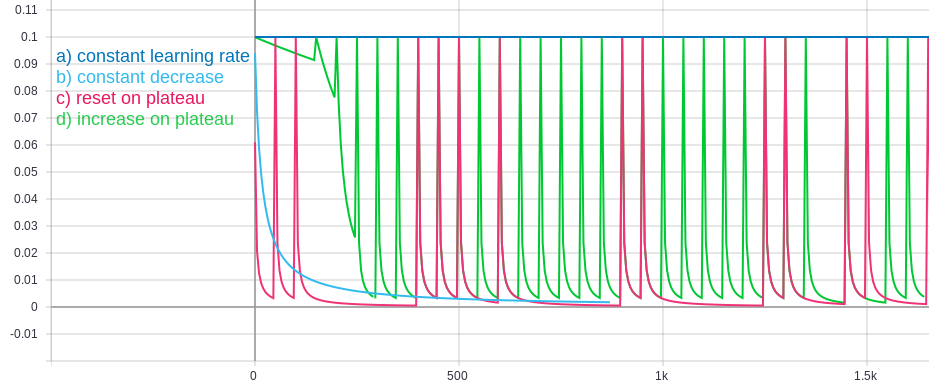
\includegraphics[width=\textwidth,height=\textheight,keepaspectratio]{img/learning_rate2.png}
    \decoRule
    \caption[Experiments: Learning Rate SGD]{Experiments with Learning Rate SGD.}
    \label{fig:sgd-learning-rate}
\end{figure}
In our experiments we tested SGD, Adam, and Nadam all with initial learning rates of $\eta=0.001$.
We configured SGD to use Nesterov Momentum with a value of $\gamma=0.9$, Adam with epsilon $\epsilon=1e-7$ and AMSGrad.
Nadam used the exponential decay parameters $\beta_1=0.9; \beta_2=0.999$ and epsilon $\epsilon=1e-7$.
Additionally, we conducted several tests with the learning rate in SGD and its influence on the training process.
One SGD configuration is with a constant learning rate $\eta$, one decays with $\eta=0.01$, and one learning rate
decays with $\eta=0.01$, but will reset to the initial learning rate, when no significant learning or changes regarding
the loss value is observed over the last 50 epochs anymore.
Another experiment with SGD increases the ascent of decay when a plateau is hit with increasing decay values
$[1e-5, 1e-4, 1e-3, 1e-2]$ as visualized in ~\ref{fig:sgd-learning-rate}.



% https://ruder.io/optimizing-gradient-descent/index.html#nadam

%The goal of gradient descent is to find the minima of the weights, so that the overall error is minimized.
%
%The learning rate is one of the important hyper-parameters, which determines how quickly this minimum can be reached.
%It sets the step size and with it the amount of steps until the model converges.
%So it additionally decides about the training length of the network~\cite{deeplcomputervision}.




%https://mlfromscratch.com/optimizers-explained/#/

\subsubsection*{Comparison of Adam, Nadam and SGD}
\begin{figure}[H]
    \centering
    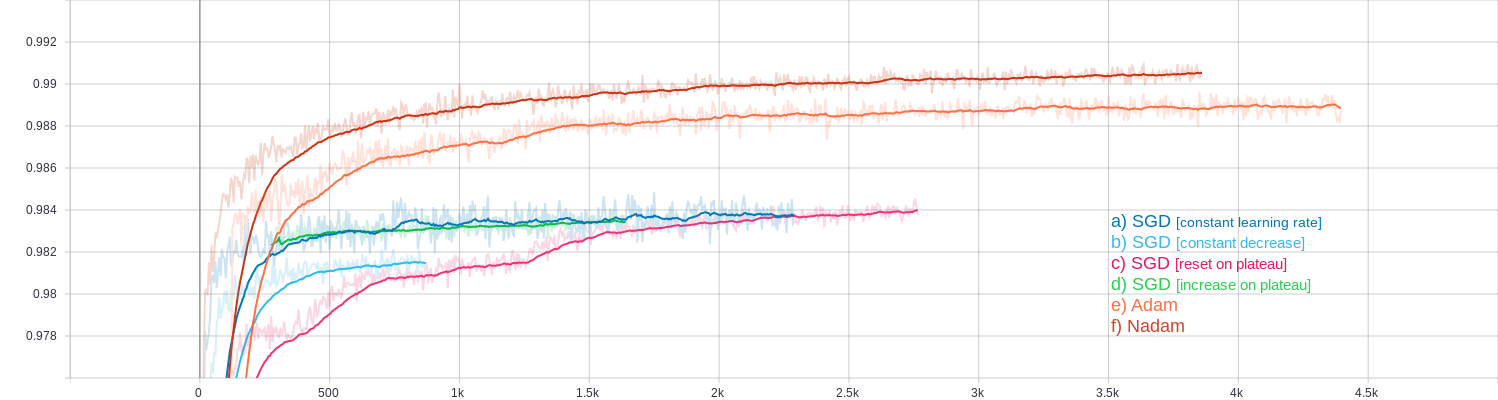
\includegraphics[width=\textwidth,height=\textheight,keepaspectratio]{img/accuracy_all.png}
    \decoRule
    \caption[Experiments: Accuracy]{Accuracy of different optimizer settings}
    \label{fig:accuracy}
\end{figure}

The Figure on accuracy~\ref{fig:accuracy} shows that our network makes huge learn progress in the first
200 to 300 epochs with an ascent of almost 90 degrees.
However, the graph shows that SGD performs worse than Adam or Nadam, all networks reach a commendable accuracy above
98 percent, whereas Nadam even gets over the 99 percent mark.
Adam and Nadam start to flatten a little bit later than SGD about 100 epochs.
Furthermore, their curves flatten more evenly, whereas SGD
seems to flatten more abruptly.
Interestingly, the SGD optimizer, where we reset the learning rate on plateau, shows jumps in its curve.
There one can observe the typical flattening of SGD and then, when a reset took place, the learning process starts again.
This indicates that SGD hit local minima from which it seems to jump out and re-trigger the adjustment of $\theta$.

%\begin{figure}[H]
%    \centering
%    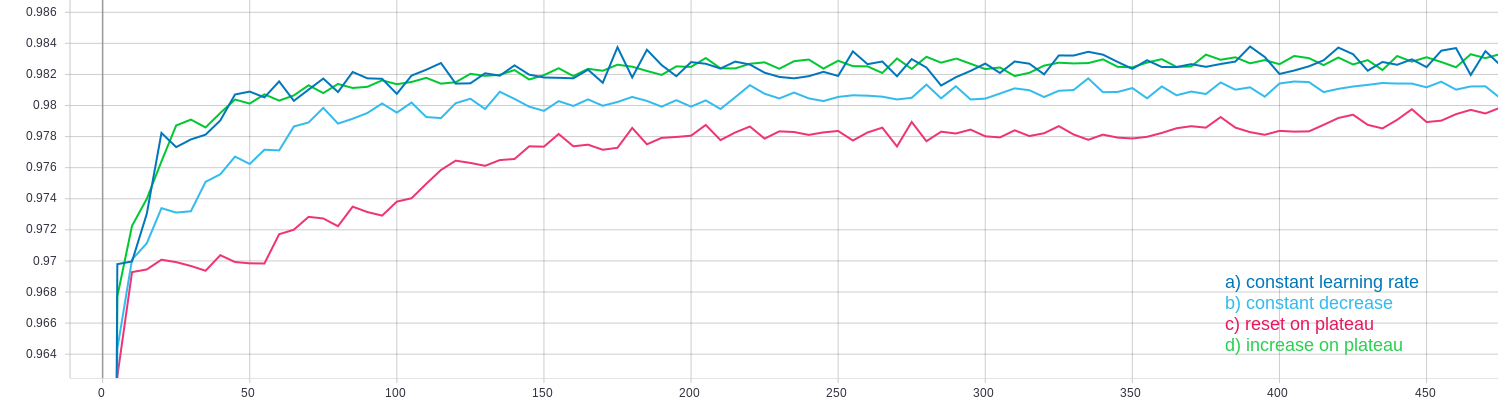
\includegraphics[width=\textwidth,height=\textheight,keepaspectratio]{img/accuracy_sgd.png}
%    \decoRule
%    \caption[Accuracy SGD]{Accuracy SGD.}
%    \label{fig:sgd-accuracy}
%\end{figure}



%\begin{figure}[H]
%    \centering
%    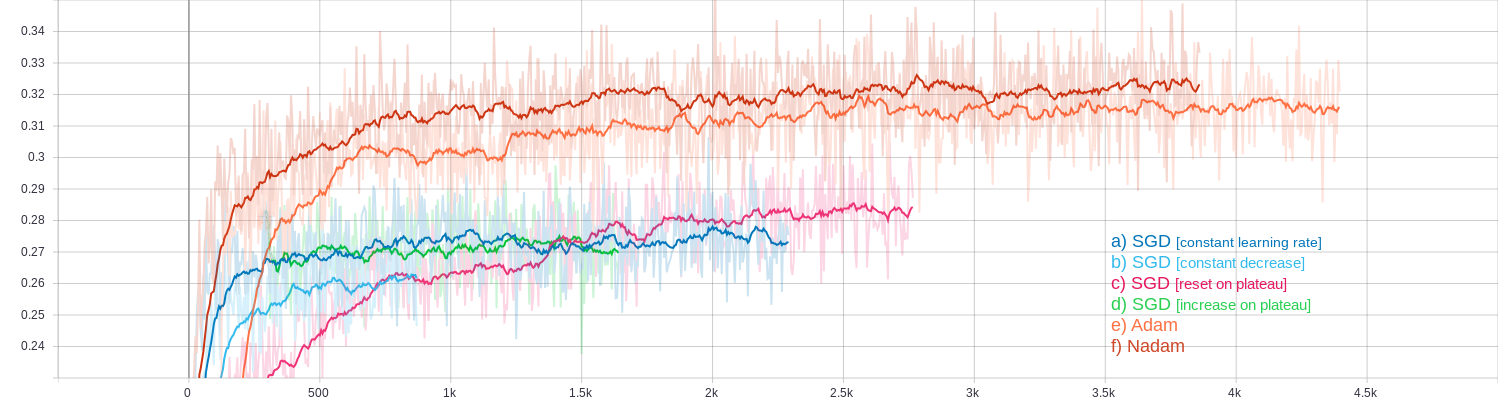
\includegraphics[width=\textwidth,height=\textheight,keepaspectratio]{img/accuracy_body_part_all.png}
%    \decoRule
%    \caption[Correct BPR]{Correct body part pixel relation}
%    \label{fig:acc-bp}
%\end{figure}


\begin{figure}[H]
    \centering
    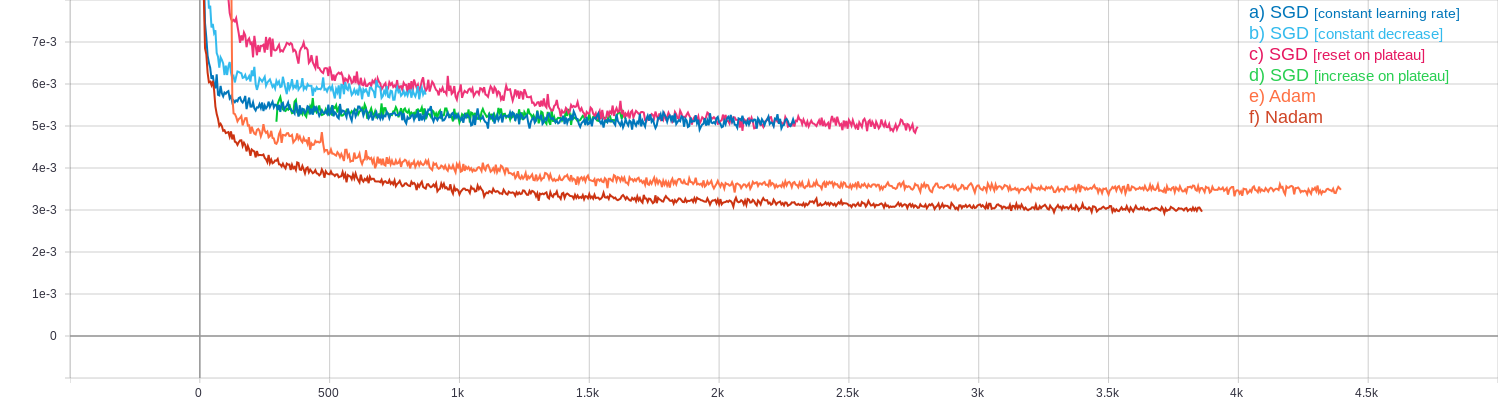
\includegraphics[width=\textwidth,height=\textheight,keepaspectratio]{img/loss_all.png}
    \decoRule
    \caption[Experiments: Loss curves]{Experiments: Loss curves}
    \label{fig:loss}
\end{figure}
Similar process curve trends can be observed in~\ref{fig:loss}, while the curves are mirrored at the x-axis.
This correlation of loss and accuracy trend proves the associate learning process for the different optimizers.
\\\mbox{}\\
\paragraph{Conclusions}\mbox{}\\
Our results are reflected by the research from Choi et Al~\cite{empiricaloptimizers}.
They conducted very interesting research with the thesis that more general optimizers would never underperform
the ones they approximate.
Meaning RMSProp, Adam and Nadam would always perform at least as good if not better than Momentum, Nesterov or SGD.
They impose to carefully tune the hyperparameters and not just conclude an optimizer would work better than another one.
This is why we used very commonly recommended hyperparameters.
A continuing grid search could help to find an even more efficient way for training and probably even result in better
learned network parameters $\theta$.
%\begin{figure}[H]
%    \centering
%    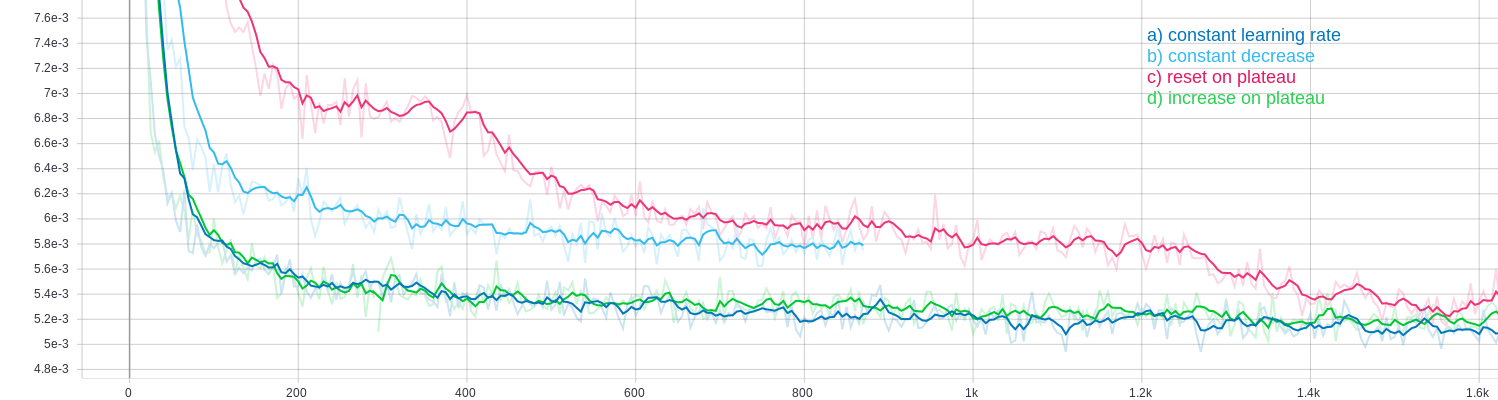
\includegraphics[width=\textwidth,height=\textheight,keepaspectratio]{img/loss_sgd.png}
%    \decoRule
%    \caption[Loss SGD]{Loss SGD.}
%    \label{fig:sgd-loss}
%\end{figure}



%----------------------------------------------------------------------------------------
%	SECTION 3
%----------------------------------------------------------------------------------------


\section{Performance of loss functions}

As already mentioned in~\autoref{optimizers} loss functions $\mathfrak{J}$ closely work together with optimizer algorithms.
The loss function is used in the optimizer algorithm as seminal feedback deciding about the success of the learning process of a
neural network.
It calculates how close a prediction $y_p$ from a neural network is to the true label $y_t$.

\subsection{Commonly used loss functions}
One classical loss function is Mean Squared Error (MSE).
The error represents the difference between $y_t$ and $y_p$.
MSE then squares the error to even out negative results and calculates the sum of all these errors.
For our fully convolutional network, each pixel presents a certain class.
As visualized in~\ref{fig:feature-maps-output}, our Human Parts module predicts nine classes.
This means, there are nine labels possible for each pixel.
Now, the neural network estimates with a certain probability of how likely a certain class would be true for a specific pixel.
The error then calculates the difference between the estimation or prediction and the true label, which includes a
value of 1 only for the true class.
Additionally to the summation of squared errors, MSE divides this sum with the number of all squares resulting in the mean
value:

\begin{align}
    MSE(y_t,y_p) = \frac{1}{n}\cdot\sum_[i=1]^n(y_t-y_p)^2
\end{align}

We trained the Keypoint Detection and Body Part Extraction modules with MSE.

However, with our Body Part Detection Module we initially had problems with class imbalances.
First, we conducted our training with Sparse Categorical Cross Entropy (SCCE), which is a common loss function used in image
segmentation.
Wrong predictions are weighed harder, especially the ones with a great wrong probability value.
This is accomplished by calculating the logarithm of the predicted values.
Since the logarithm function $log(x)$ is negative for $x \in \Re and [0>x>1]$, and input values closer to zero mean
an exponential decrease towards $-\infty$ and there is just one true label for the different classes of one pixel, if
the prediction is clearly the wrong class, the cost will be exponentially higher.

\begin{align}
    SCCE(y_t,y_p) = -\sum_{i,j=1}^{i,j}y_{t_{i,j}}\cdot log(y_{p_{i,j}})
\end{align}
Here \textit{i,j} stands for the column and row pixels of the image.

Nevertheless, our first results~\ref{fig:cross_entropy_pred_img} made us believe that with SCCE our net was not able to
learn the correct labels for the pixels.
Especially the prediction after the 60th epoch shows, that the net mainly has learned to classify all body parts with the
torso class.
We assumed this was the case, because the likeliness of the pixel to be of class torso is higher than, for
example, foot.
Furthermore, however, the accuracy graph shows descent results over 94 percent it started to flatten more and more becoming
almost flat after the 50th epoch already.
\begin{figure}[H]
    \centering
    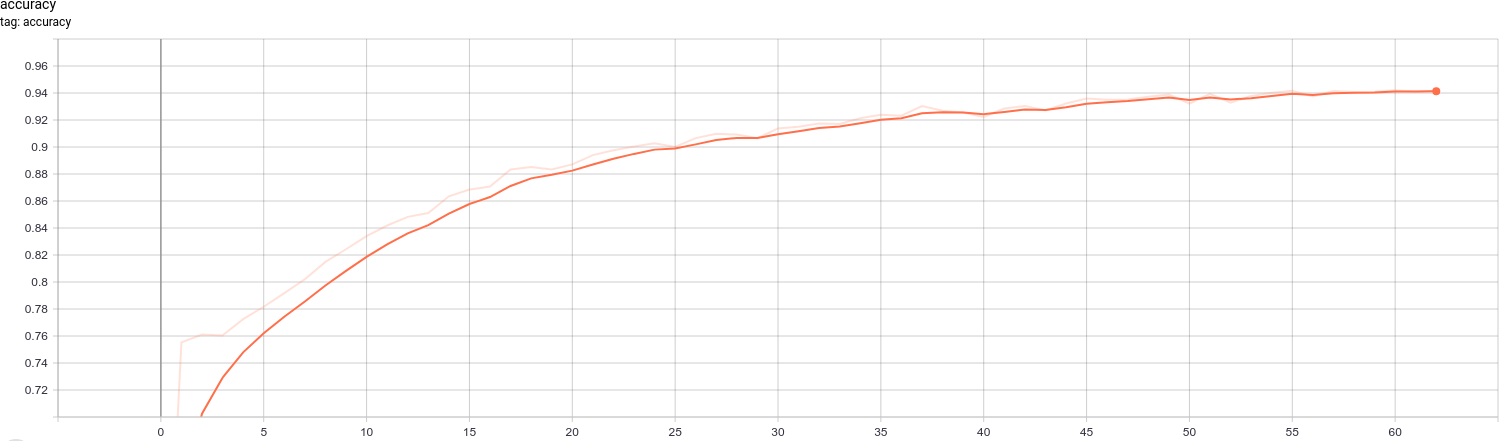
\includegraphics[width=\textwidth,height=\textheight,keepaspectratio]{Figures/accuracy_cross_entropy.png}
    \decoRule
    \caption[Loss Functions SCCE: Accuracy]{Accuracy for training with Sparse Categorical Cross Enntropy loss function}
    \label{fig:accuracy_cross_entropy}
\end{figure}
\begin{figure}[H]
    \centering
    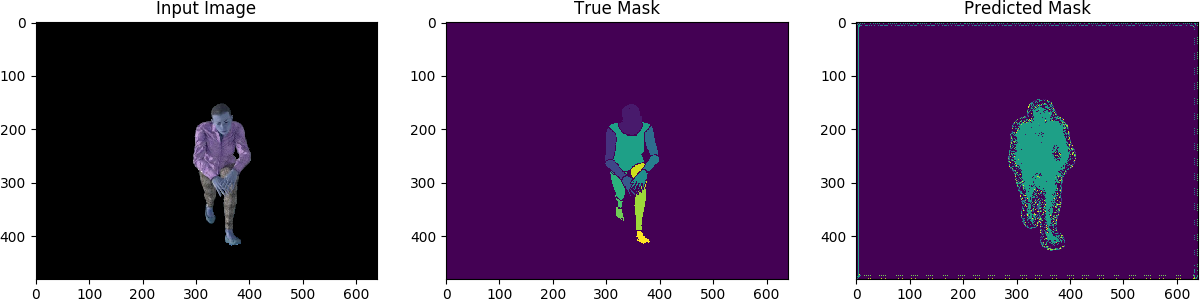
\includegraphics[width=\textwidth,height=\textheight,keepaspectratio]{Figures/crossentropy_imgs_prediction_last_epoch.png}
    \decoRule
    \caption[Loss Functions SCCE: predictions]{Predicted images for training with Sparse Categorical Cross Entropy loss function}
    \label{fig:cross_entropy_pred_img}
\end{figure}
We than created our own loss function for this class imbalance problem as explained in~\autoref{ciloss}.
Moreover, we reduced the number of classes from 14 to nine accumulating left and right body parts such as foot and arm.
A later experiment shows, on the contrary, that our build network HRNetv3 even learns slightly better than with our own created
loss function CILoss~\ref{fig:ablation-accuracy}.
Even though, this of course could be by chance due to current training circumstances.


\subsection{Our custom loss function CILoss}
\label{ciloss}
This loss function confronts the problem of class imbalance, which especially occurs in body part recognition.
The background pixels appear most often, and the different body part classes occur much less often and they even
differ a lot in their relative occurrence.
\\\mbox{}\\
We try to confront this problem with a weighed map $\mu$, which takes the body parts as a graph and calculates
the distances from each body part $b_x$ to all other body parts $b_n$, and store this data inside a table.
This weighed map $\mu$ is applied to the true labels of $y_{true}$ so that wrong predictions further away from the true
class will be punished more. For example if the network predicts hand instead of lower arm, the error will be less as if
the network predicts foot.
\\\mbox{}\\
Additionally, this weight map is evened out with a multiplier to reduce the distances and facilitate
the learning process for the network.
\\\mbox{}\\
As in MSE we calculate the difference $\mathcal{E}$ between $y_t$ and $y_p$, but do not square the result, we just use the absolute value.
We multiply the resulting error $\mathcal{E}$ with our weighed map receiving $\delta$.
To calculate the loss we then sum the error $\mathcal{E}$ and delta $\delta$ pixel-wise:

$$\mathcal{E}=y_t(x)-y_p(x)$$
$$\delta=\theta\cdot\mu[argmax(y_t)] $$
$$L=\sum_{i=0}^{n}\mathcal{E}_i+\delta_i$$


\begin{figure}[H]
    \centering
    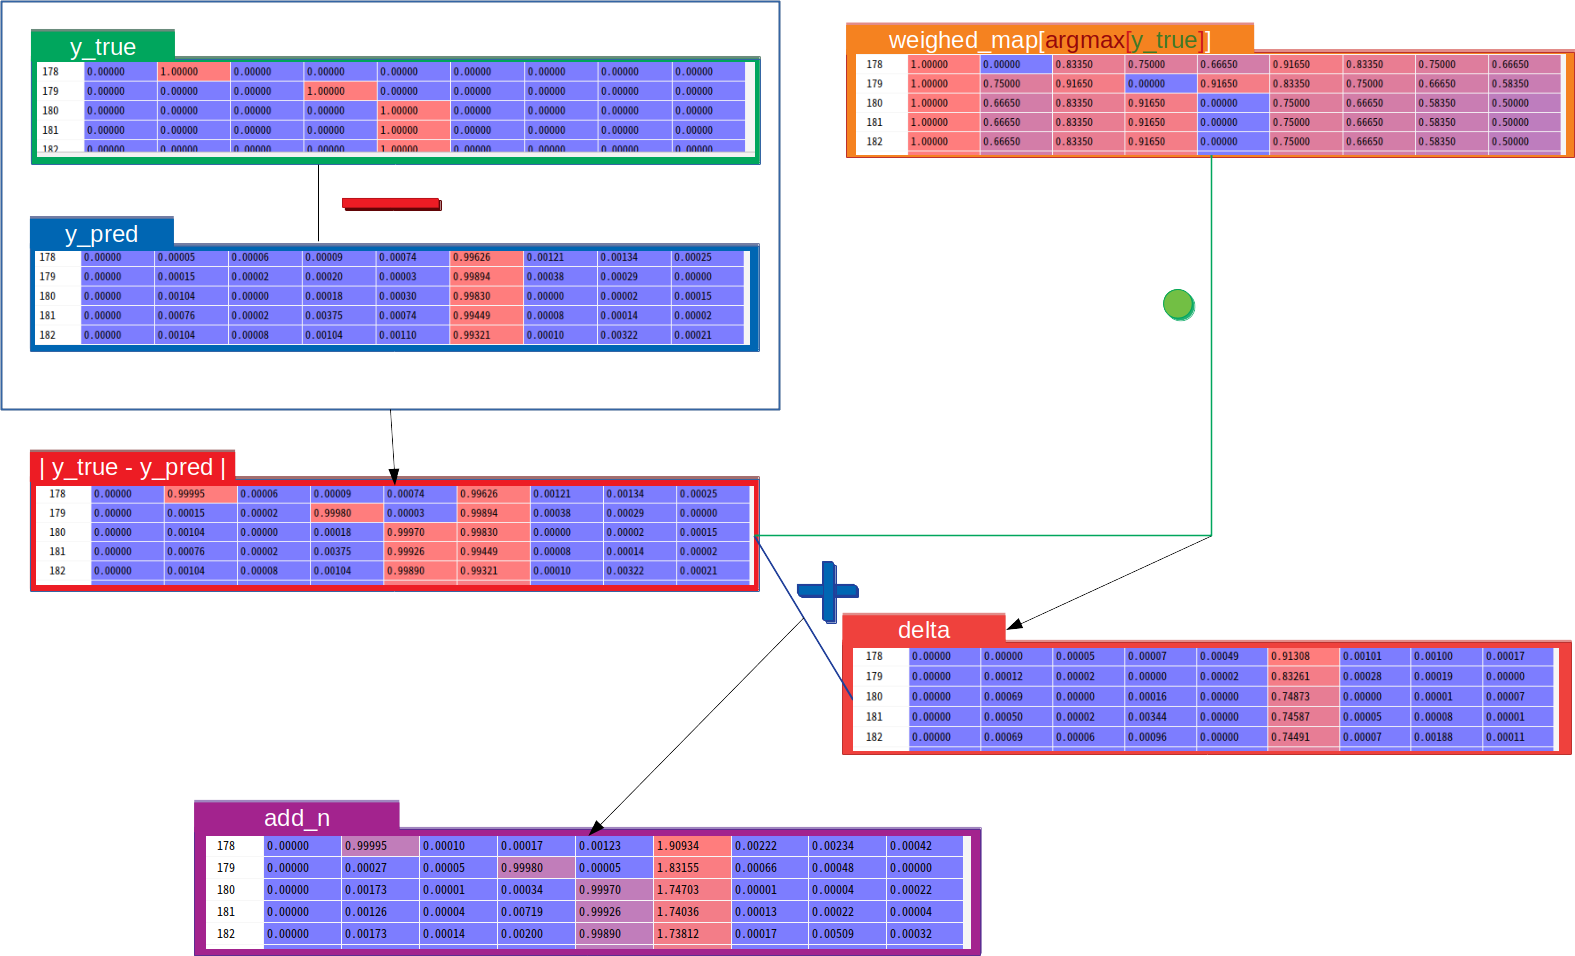
\includegraphics[width=\textwidth,height=\textheight,keepaspectratio]{img/loss_calculation.png}
    \decoRule
    \caption[Loss Functions CILoss: Calculation]{Visualization of our custom loss function CILoss}
    \label{fig:ciloss-calc}
\end{figure}

%! Author = nadin-katrin
%! Date = 03.04.20
\chapter{Conclusion and future thoughts}
\label{conclusion}
Inspired by popular research from \textit{OpenPose, VidePose3d} or \textit{Simulation of figure skating} ~\cite{openpose, videopose3d, figureskatingsimulation}
which all have problems to correctly predict human joint locations for spins in figure ice skating, this thesis analyzed
several aspects such as motion capture with connection to dataset creation techniques and network architectures with influence of optimizer and loss functions.
\\\mbox{}\\
The result of this research work is a successfully created new high resolution fully convolutional neural network HRNetv3, which includes state-of-the-art
research findings from I.a. HRNet, HRNetV2, and MobileNet~\cite{HRNetv1, HRNetv2, mobilenet}.
This algorithm accomplished to predict human joint locations by learning from the synthetic dataset 3DPeople~\cite{3dpeople}.
In sum, three modules for background extraction, human parts detection, and keypoint recognition were created.
These modules partly correspond to concepts used in other state-of-the-art research such as \textit{OpenPose}, however, the
single ice skating domain specific background extraction module stands out other architectures.
\\\mbox{}\\
For the applied research, a Python 3.7 project  was built with Tensorflow 2~\cite{tensorflow2} as core library.
Several experiments were performed in multiple Docker containers with the Tensorflow:\textit{latest-devel-gpu} as base
image~\cite{tensorflowdocker}
In fact, lots of efforts was spent to write good readable code with a decent OO-style following the \textit{SOLID} principle.
So our Github repository, which is planned to be made publicly available, might help to promote further research in this topic.
Especially, the in this work used feature-driven approach making use of Github's feature pull request style and the formulation of proper
commit messages helped to iteratively improve our project architecture in a continuous style.
\\\mbox{}\\
Since the data is one of the main aspects deciding whether a neural network learns the desired predictions, a look at
motion capturing was taken and the generation of an according dataset investigated.
Further, an appropriate figure ice skating dataset for human joint recognition did not exist at the writing time of this thesis.
Some recordings were captured with the inertial motion capturing set from XSens.
The setup felt very time-consuming and the cables all over the body connected to the battery and sensors felt very uncomfortable
for the skaters on the ice.
Additionally, multiple calibrations had to be conducted, probably because the system was not prepared
for the typical gliding movements on the ice surface.
Nevertheless, after the imposing capture, the integration into Blender and use of MakeHuman for creating a synthetic dataset
became very promising.
Especially the diversity of data or video sequences possible from just one motion capture recording is highly valuable.
This is why it is very convincing that this is the way to gain decent data for an artistic sport such as figure
ice skating.
Yet, whey critically reviewing \textit{3DPeople}, where they used random background images which they put behind the moving actors,
results could improve, if an ice arena simulation was added to Blender, producing even more realistic scenes.
Another encountered caveat regarding spins was the huge amount of motion blurriness especially for skaters with high levels such as olympic or world championships winning
Evgenia Medvedeva or Alina Zagitova~\cite{2018world}.
Nevertheless, the data from \textit{3DPeople} included only image sequences without any blurriness, being one of the reasons why
the algorithm has difficulties to correctly predict human joints for spins such as the Biellmann pirouette.
\\\mbox{}\\
Throughout this research, further ideas on how to continue in this topic of human joint recognition arose.
First, creating a decent synthetic dataset for figure ice skating adding motion blurriness and improving the recorded scene
in Blender.\\
Furthermore, test other motion capturing methods as for example the \textit{Awinda} set from XSens, which could be much more comfortable
and faster to apply, because the sensors are wireless, and no cables restricting movements on the ice, must be dealt with.
Additionally, tests could be conducted with a markerless system such as Vicon~\cite{mocapoptical}.
\\\mbox{}\\%%%%
Our network architecture could become more compact and better in performance by applying a grid search with multiple different
parameters.
Moreover, the temporal information from a video could add additional information, allowing to faster and more efficiently
predict videos as already argued in ~\cite{staf}.
\\\mbox{}\\
With this here presented study we try to further spur development and research in figure ice skating to improve
fairness in this sport.
For example, in\cite{figureskatingsimulation}, they simulated some figure ice skating figures and translated these to 3d
animation. It would be very interesting to see, how skaters were rated, if the technical specialists and judges would see
the animation, without knowing, who the skater was, or what the skater looked like.
This could be a huge step in fairness.
In addition, the rating could be conducted remotely, saving the jury from the cold
ice rink and driving efforts.\\
An even more advanced step to replace the necessity of jury, who are sometimes hard to get for a competition, would be another
highly interesting research topic regarding action recognition.
Another application would be the support during practice, with recommending actions to improve some jumps for example.
\\\mbox{}\\
All in all, the here presented research is meant to serve as a foundation for further investigations towards action recognition
in sports, especially artistic ones such as figure ice skating.
Indeed, a very up-to-date topic on the writing of this paper are restrictions during the lock-downs of cities due to the
COVID-19 (Corona) virus.
Highly promising topics include as well physiotherapy or feedback during fitness and dance routines.

%\include{Chapters/Chapter4}
%\include{Chapters/Chapter5}

%----------------------------------------------------------------------------------------
%	THESIS CONTENT - APPENDICES
%----------------------------------------------------------------------------------------

\appendix % Cue to tell LaTeX that the following "chapters" are Appendices

% Include the appendices of the thesis as separate files from the Appendices folder
% Uncomment the lines as you write the Appendices

%% Appendix A

\chapter{Frequently Asked Questions} % Main appendix title

\label{AppendixA} % For referencing this appendix elsewhere, use \ref{AppendixA}

\section{How do I change the colors of links?}

The color of links can be changed to your liking using:

{\small\verb!\hypersetup{urlcolor=red}!}, or

{\small\verb!\hypersetup{citecolor=green}!}, or

{\small\verb!\hypersetup{allcolor=blue}!}.

\noindent If you want to completely hide the links, you can use:

{\small\verb!\hypersetup{allcolors=.}!}, or even better: 

{\small\verb!\hypersetup{hidelinks}!}.

\noindent If you want to have obvious links in the PDF but not the printed text, use:

{\small\verb!\hypersetup{colorlinks=false}!}.

%\include{Appendices/AppendixB}
%\include{Appendices/AppendixC}

%----------------------------------------------------------------------------------------
%	BIBLIOGRAPHY
%----------------------------------------------------------------------------------------

\printbibliography[heading=bibintoc]

%----------------------------------------------------------------------------------------
\endgroup
\end{document}
